% ==================== %
% == RESOURCES USED == %
% ==================== %


\begin{filecontents*}[overwrite]{gallery-showcase-bw.tex}
\documentclass[theme = bw]{tutodoc}

% -- FORDOC -- %

\usepackage[french]{babel}
\frenchsetup{StandardItemLabels=true}

\usepackage{multicol}
\usepackage{lastpage}

\makeatletter

\renewcommand*\pagemark{%
  	\usekomafont{pagenumber}{%
  		\thepage\kern1pt/\kern1pt\pageref*{LastPage}%
	}%
}

\makeatother


\newcommand\thisstyle{bw}


\newcommand\myexrmktext{
    \tdocversion{1.7.0}[2024-12-04]
    Dans le flot du texte, il est toujours utile de pouvoir indiquer des exemples et des remarques qui viennent compléter le contenu principal.
}


\newcommand\myadmotext{
    Suivant le contexte d'utilisation, il est parfois nécessaire de pouvoir mettre en avant des contenus en indiquant leur degré d'importance.
}

\newcommand\myhighlightedtextnonote{
    Que dire ?
    Je ne sais pas, mais c'est sympathique. Non ?
}

\newcommand\myhighlightedtext{
    Que dire\,%
    \footnote{
        N'oublions pas les notes de bas de page...
    }?
    Je ne sais pas, mais c'est sympathique. Non ?
}


\newcommand\mychgestext{
    Dans un journal de bord, il est important de bien visualiser les types de changements. Ceci rend plus efficace la lecture côté utilisateur !
}


\ExplSyntaxOn

\int_new:N \g__tutodoc_for_doc_int

\ExplSyntaxOff


\begin{document}

\textsf{\Huge\bfseries Le thème \texttt{"\thisstyle"}}

\section{Liens}

{\Large\bfseries \href{https://github.com/bc-tools/for-latex/tree/main/tutodoc}{Un lien très gros}}, mais au moins on le voit.



\section{Des codes \LaTeX}

Taper du code \LaTeX\ en ligne comme \tdoclatexin{E = m c^2 \neq \pi \neq \frac{3}{14}} est utile, tout comme montrer des cas d'utilisation comme le suivant.

\begin{tdoclatex}
Du code \LaTeX\ mis en forme, c'est top : $E = m c^2$ ou $\pi \neq \frac{3}{14}$.
\end{tdoclatex}


On dispose aussi d'un mode côte-à-côte moins envahissant. Sympa ! Non ?

\begin{tdoclatex}<\tdoctcb{sbs}>
Du code \LaTeX\ mis en forme, c'est top : \\
$E = m c^2$ ou $\pi \neq \frac{3}{14}$.
\end{tdoclatex}



\section{Mettre en avant, versionner et dater}

\subsection{tdocexa, tdocrem}

\myexrmktext

\ExplSyntaxOn

\seq_map_inline:Nn \g__tutodoc_focus_std_seq {
    \begin{tdoc#1}
        \myhighlightedtext
    \end{tdoc#1}
}

\ExplSyntaxOff



\subsection{tdocnote, tdoctip...}

\myadmotext

\ExplSyntaxOn

\int_set:Nn \g__tutodoc_for_doc_int { 0 }

\ifcsundef{g__tutodoc_focus_color_seq}{
    \prop_map_inline:Nn \g__tutodoc_focus_color_prop {
        \int_gincr:N \g__tutodoc_for_doc_int

        \begin{tdoc#1}
      	  	\int_compare:nTF
	    		{\g__tutodoc_for_doc_int = 1 }
	    		{ \myhighlightedtext }
	    		{ \myhighlightedtextnonote }
        \end{tdoc#1}
    }
} {
    \seq_map_inline:Nn \g__tutodoc_focus_color_seq {
        \int_gincr:N \g__tutodoc_for_doc_int

        \begin{tdoc#1}
      	  	\int_compare:nTF
	    		{\g__tutodoc_for_doc_int = 1 }
	    		{ \myhighlightedtext }
	    		{ \myhighlightedtextnonote }
        \end{tdoc#1}
    }
}

\ExplSyntaxOff



\subsection{tdocbreak, tdocfix...}

\tdocstartproj{Une nouvelle section démonstrative...}

\begin{tdoctodo}
	\item Une galerie serait bienvenue...
\end{tdoctodo}

\ifcsundef{g__tutodoc_topic_change_seq}{
 	\medskip
}{}

\mychgestext

\ifcsundef{g__tutodoc_topic_change_seq}{
	\medskip
}{}

\ExplSyntaxOn

\int_set:Nn \g__tutodoc_for_doc_int { 0 }

\begin{tabular}{%
	@{\hskip 0pt}p{.26\linewidth}%
	*{3}{@{\hskip 7pt}p{.23\linewidth}}@{\hskip 0pt}%
}
	\ifcsundef{g__tutodoc_topic_change_seq}{
    	\prop_map_inline:Nn \g__tutodoc_topic_change_prop {
          	\int_gincr:N \g__tutodoc_for_doc_int

          	\vspace{-12pt}

    	  	\begin{tdoc#1}
           		\item Infos...
    	  	\end{tdoc#1}

    	  	\int_compare:nTF
    	    	{\g__tutodoc_for_doc_int = 4 }
    	    	{ \\ }
    	    	{ & }
    	}
	}{
    	\seq_map_inline:Nn \g__tutodoc_topic_change_seq {
          	\int_gincr:N \g__tutodoc_for_doc_int

          	\vspace{-5pt}

    	  	\begin{tdoc#1}
           		\item Infos...
    	  	\end{tdoc#1}

    	  	\int_compare:nTF
    	    	{\g__tutodoc_for_doc_int = 4 }
    	    	{ \\ }
    	    	{ & }
    	}
	}
\end{tabular}

\ExplSyntaxOff

\end{document}

\end{filecontents*}

\begin{filecontents*}[overwrite]{gallery-showcase-color.tex}
\documentclass[theme = color]{tutodoc}

% -- FORDOC -- %

\usepackage[french]{babel}
\frenchsetup{StandardItemLabels=true}

\usepackage{multicol}
\usepackage{lastpage}

\makeatletter

\renewcommand*\pagemark{%
  	\usekomafont{pagenumber}{%
  		\thepage\kern1pt/\kern1pt\pageref*{LastPage}%
	}%
}

\makeatother


\newcommand\thisstyle{color}


\newcommand\myexrmktext{
    \tdocversion{1.7.0}[2024-12-04]
    Dans le flot du texte, il est toujours utile de pouvoir indiquer des exemples et des remarques qui viennent compléter le contenu principal.
}


\newcommand\myadmotext{
    Suivant le contexte d'utilisation, il est parfois nécessaire de pouvoir mettre en avant des contenus en indiquant leur degré d'importance.
}

\newcommand\myhighlightedtextnonote{
    Que dire ?
    Je ne sais pas, mais c'est sympathique. Non ?
}

\newcommand\myhighlightedtext{
    Que dire\,%
    \footnote{
        N'oublions pas les notes de bas de page...
    }?
    Je ne sais pas, mais c'est sympathique. Non ?
}


\newcommand\mychgestext{
    Dans un journal de bord, il est important de bien visualiser les types de changements. Ceci rend plus efficace la lecture côté utilisateur !
}


\ExplSyntaxOn

\int_new:N \g__tutodoc_for_doc_int

\ExplSyntaxOff


\begin{document}

\textsf{\Huge\bfseries Le thème \texttt{"\thisstyle"}}

\section{Liens}

{\Large\bfseries \href{https://github.com/bc-tools/for-latex/tree/main/tutodoc}{Un lien très gros}}, mais au moins on le voit.



\section{Des codes \LaTeX}

Taper du code \LaTeX\ en ligne comme \tdoclatexin{E = m c^2 \neq \pi \neq \frac{3}{14}} est utile, tout comme montrer des cas d'utilisation comme le suivant.

\begin{tdoclatex}
Du code \LaTeX\ mis en forme, c'est top : $E = m c^2$ ou $\pi \neq \frac{3}{14}$.
\end{tdoclatex}


On dispose aussi d'un mode côte-à-côte moins envahissant. Sympa ! Non ?

\begin{tdoclatex}<\tdoctcb{sbs}>
Du code \LaTeX\ mis en forme, c'est top : \\
$E = m c^2$ ou $\pi \neq \frac{3}{14}$.
\end{tdoclatex}



\section{Mettre en avant, versionner et dater}

\subsection{tdocexa, tdocrem}

\myexrmktext

\ExplSyntaxOn

\seq_map_inline:Nn \g__tutodoc_focus_std_seq {
    \begin{tdoc#1}
        \myhighlightedtext
    \end{tdoc#1}
}

\ExplSyntaxOff



\subsection{tdocnote, tdoctip...}

\myadmotext

\ExplSyntaxOn

\int_set:Nn \g__tutodoc_for_doc_int { 0 }

\ifcsundef{g__tutodoc_focus_color_seq}{
    \prop_map_inline:Nn \g__tutodoc_focus_color_prop {
        \int_gincr:N \g__tutodoc_for_doc_int

        \begin{tdoc#1}
      	  	\int_compare:nTF
	    		{\g__tutodoc_for_doc_int = 1 }
	    		{ \myhighlightedtext }
	    		{ \myhighlightedtextnonote }
        \end{tdoc#1}
    }
} {
    \seq_map_inline:Nn \g__tutodoc_focus_color_seq {
        \int_gincr:N \g__tutodoc_for_doc_int

        \begin{tdoc#1}
      	  	\int_compare:nTF
	    		{\g__tutodoc_for_doc_int = 1 }
	    		{ \myhighlightedtext }
	    		{ \myhighlightedtextnonote }
        \end{tdoc#1}
    }
}

\ExplSyntaxOff



\subsection{tdocbreak, tdocfix...}

\tdocstartproj{Une nouvelle section démonstrative...}

\begin{tdoctodo}
	\item Une galerie serait bienvenue...
\end{tdoctodo}

\ifcsundef{g__tutodoc_topic_change_seq}{
 	\medskip
}{}

\mychgestext

\ifcsundef{g__tutodoc_topic_change_seq}{
	\medskip
}{}

\ExplSyntaxOn

\int_set:Nn \g__tutodoc_for_doc_int { 0 }

\begin{tabular}{%
	@{\hskip 0pt}p{.26\linewidth}%
	*{3}{@{\hskip 7pt}p{.23\linewidth}}@{\hskip 0pt}%
}
	\ifcsundef{g__tutodoc_topic_change_seq}{
    	\prop_map_inline:Nn \g__tutodoc_topic_change_prop {
          	\int_gincr:N \g__tutodoc_for_doc_int

          	\vspace{-12pt}

    	  	\begin{tdoc#1}
           		\item Infos...
    	  	\end{tdoc#1}

    	  	\int_compare:nTF
    	    	{\g__tutodoc_for_doc_int = 4 }
    	    	{ \\ }
    	    	{ & }
    	}
	}{
    	\seq_map_inline:Nn \g__tutodoc_topic_change_seq {
          	\int_gincr:N \g__tutodoc_for_doc_int

          	\vspace{-5pt}

    	  	\begin{tdoc#1}
           		\item Infos...
    	  	\end{tdoc#1}

    	  	\int_compare:nTF
    	    	{\g__tutodoc_for_doc_int = 4 }
    	    	{ \\ }
    	    	{ & }
    	}
	}
\end{tabular}

\ExplSyntaxOff

\end{document}

\end{filecontents*}

\begin{filecontents*}[overwrite]{gallery-showcase-dark.tex}
\documentclass[theme = dark]{tutodoc}

% -- FORDOC -- %

\usepackage[french]{babel}
\frenchsetup{StandardItemLabels=true}

\usepackage{multicol}
\usepackage{lastpage}

\makeatletter

\renewcommand*\pagemark{%
  	\usekomafont{pagenumber}{%
  		\thepage\kern1pt/\kern1pt\pageref*{LastPage}%
	}%
}

\makeatother


\newcommand\thisstyle{dark}


\newcommand\myexrmktext{
    \tdocversion{1.7.0}[2024-12-04]
    Dans le flot du texte, il est toujours utile de pouvoir indiquer des exemples et des remarques qui viennent compléter le contenu principal.
}


\newcommand\myadmotext{
    Suivant le contexte d'utilisation, il est parfois nécessaire de pouvoir mettre en avant des contenus en indiquant leur degré d'importance.
}

\newcommand\myhighlightedtextnonote{
    Que dire ?
    Je ne sais pas, mais c'est sympathique. Non ?
}

\newcommand\myhighlightedtext{
    Que dire\,%
    \footnote{
        N'oublions pas les notes de bas de page...
    }?
    Je ne sais pas, mais c'est sympathique. Non ?
}


\newcommand\mychgestext{
    Dans un journal de bord, il est important de bien visualiser les types de changements. Ceci rend plus efficace la lecture côté utilisateur !
}


\ExplSyntaxOn

\int_new:N \g__tutodoc_for_doc_int

\ExplSyntaxOff


\begin{document}

\textsf{\Huge\bfseries Le thème \texttt{"\thisstyle"}}

\section{Liens}

{\Large\bfseries \href{https://github.com/bc-tools/for-latex/tree/main/tutodoc}{Un lien très gros}}, mais au moins on le voit.



\section{Des codes \LaTeX}

Taper du code \LaTeX\ en ligne comme \tdoclatexin{E = m c^2 \neq \pi \neq \frac{3}{14}} est utile, tout comme montrer des cas d'utilisation comme le suivant.

\begin{tdoclatex}
Du code \LaTeX\ mis en forme, c'est top : $E = m c^2$ ou $\pi \neq \frac{3}{14}$.
\end{tdoclatex}


On dispose aussi d'un mode côte-à-côte moins envahissant. Sympa ! Non ?

\begin{tdoclatex}<\tdoctcb{sbs}>
Du code \LaTeX\ mis en forme, c'est top : \\
$E = m c^2$ ou $\pi \neq \frac{3}{14}$.
\end{tdoclatex}



\section{Mettre en avant, versionner et dater}

\subsection{tdocexa, tdocrem}

\myexrmktext

\ExplSyntaxOn

\seq_map_inline:Nn \g__tutodoc_focus_std_seq {
    \begin{tdoc#1}
        \myhighlightedtext
    \end{tdoc#1}
}

\ExplSyntaxOff



\subsection{tdocnote, tdoctip...}

\myadmotext

\ExplSyntaxOn

\int_set:Nn \g__tutodoc_for_doc_int { 0 }

\ifcsundef{g__tutodoc_focus_color_seq}{
    \prop_map_inline:Nn \g__tutodoc_focus_color_prop {
        \int_gincr:N \g__tutodoc_for_doc_int

        \begin{tdoc#1}
      	  	\int_compare:nTF
	    		{\g__tutodoc_for_doc_int = 1 }
	    		{ \myhighlightedtext }
	    		{ \myhighlightedtextnonote }
        \end{tdoc#1}
    }
} {
    \seq_map_inline:Nn \g__tutodoc_focus_color_seq {
        \int_gincr:N \g__tutodoc_for_doc_int

        \begin{tdoc#1}
      	  	\int_compare:nTF
	    		{\g__tutodoc_for_doc_int = 1 }
	    		{ \myhighlightedtext }
	    		{ \myhighlightedtextnonote }
        \end{tdoc#1}
    }
}

\ExplSyntaxOff



\subsection{tdocbreak, tdocfix...}

\tdocstartproj{Une nouvelle section démonstrative...}

\begin{tdoctodo}
	\item Une galerie serait bienvenue...
\end{tdoctodo}

\ifcsundef{g__tutodoc_topic_change_seq}{
 	\medskip
}{}

\mychgestext

\ifcsundef{g__tutodoc_topic_change_seq}{
	\medskip
}{}

\ExplSyntaxOn

\int_set:Nn \g__tutodoc_for_doc_int { 0 }

\begin{tabular}{%
	@{\hskip 0pt}p{.26\linewidth}%
	*{3}{@{\hskip 7pt}p{.23\linewidth}}@{\hskip 0pt}%
}
	\ifcsundef{g__tutodoc_topic_change_seq}{
    	\prop_map_inline:Nn \g__tutodoc_topic_change_prop {
          	\int_gincr:N \g__tutodoc_for_doc_int

          	\vspace{-12pt}

    	  	\begin{tdoc#1}
           		\item Infos...
    	  	\end{tdoc#1}

    	  	\int_compare:nTF
    	    	{\g__tutodoc_for_doc_int = 4 }
    	    	{ \\ }
    	    	{ & }
    	}
	}{
    	\seq_map_inline:Nn \g__tutodoc_topic_change_seq {
          	\int_gincr:N \g__tutodoc_for_doc_int

          	\vspace{-5pt}

    	  	\begin{tdoc#1}
           		\item Infos...
    	  	\end{tdoc#1}

    	  	\int_compare:nTF
    	    	{\g__tutodoc_for_doc_int = 4 }
    	    	{ \\ }
    	    	{ & }
    	}
	}
\end{tabular}

\ExplSyntaxOff

\end{document}

\end{filecontents*}

\begin{filecontents*}[overwrite]{gallery-showcase-draft.tex}
\documentclass[theme = draft]{tutodoc}

% -- FORDOC -- %

\usepackage[french]{babel}
\frenchsetup{StandardItemLabels=true}

\usepackage{multicol}
\usepackage{lastpage}

\makeatletter

\renewcommand*\pagemark{%
  	\usekomafont{pagenumber}{%
  		\thepage\kern1pt/\kern1pt\pageref*{LastPage}%
	}%
}

\makeatother


\newcommand\thisstyle{draft}


\newcommand\myexrmktext{
    \tdocversion{1.7.0}[2024-12-04]
    Dans le flot du texte, il est toujours utile de pouvoir indiquer des exemples et des remarques qui viennent compléter le contenu principal.
}


\newcommand\myadmotext{
    Suivant le contexte d'utilisation, il est parfois nécessaire de pouvoir mettre en avant des contenus en indiquant leur degré d'importance.
}

\newcommand\myhighlightedtextnonote{
    Que dire ?
    Je ne sais pas, mais c'est sympathique. Non ?
}

\newcommand\myhighlightedtext{
    Que dire\,%
    \footnote{
        N'oublions pas les notes de bas de page...
    }?
    Je ne sais pas, mais c'est sympathique. Non ?
}


\newcommand\mychgestext{
    Dans un journal de bord, il est important de bien visualiser les types de changements. Ceci rend plus efficace la lecture côté utilisateur !
}


\ExplSyntaxOn

\int_new:N \g__tutodoc_for_doc_int

\ExplSyntaxOff


\begin{document}

\textsf{\Huge\bfseries Le thème \texttt{"\thisstyle"}}

\section{Liens}

{\Large\bfseries \href{https://github.com/bc-tools/for-latex/tree/main/tutodoc}{Un lien très gros}}, mais au moins on le voit.



\section{Des codes \LaTeX}

Taper du code \LaTeX\ en ligne comme \tdoclatexin{E = m c^2 \neq \pi \neq \frac{3}{14}} est utile, tout comme montrer des cas d'utilisation comme le suivant.

\begin{tdoclatex}
Du code \LaTeX\ mis en forme, c'est top : $E = m c^2$ ou $\pi \neq \frac{3}{14}$.
\end{tdoclatex}


On dispose aussi d'un mode côte-à-côte moins envahissant. Sympa ! Non ?

\begin{tdoclatex}<\tdoctcb{sbs}>
Du code \LaTeX\ mis en forme, c'est top : \\
$E = m c^2$ ou $\pi \neq \frac{3}{14}$.
\end{tdoclatex}



\section{Mettre en avant, versionner et dater}

\subsection{tdocexa, tdocrem}

\myexrmktext

\ExplSyntaxOn

\seq_map_inline:Nn \g__tutodoc_focus_std_seq {
    \begin{tdoc#1}
        \myhighlightedtext
    \end{tdoc#1}
}

\ExplSyntaxOff



\subsection{tdocnote, tdoctip...}

\myadmotext

\ExplSyntaxOn

\int_set:Nn \g__tutodoc_for_doc_int { 0 }

\ifcsundef{g__tutodoc_focus_color_seq}{
    \prop_map_inline:Nn \g__tutodoc_focus_color_prop {
        \int_gincr:N \g__tutodoc_for_doc_int

        \begin{tdoc#1}
      	  	\int_compare:nTF
	    		{\g__tutodoc_for_doc_int = 1 }
	    		{ \myhighlightedtext }
	    		{ \myhighlightedtextnonote }
        \end{tdoc#1}
    }
} {
    \seq_map_inline:Nn \g__tutodoc_focus_color_seq {
        \int_gincr:N \g__tutodoc_for_doc_int

        \begin{tdoc#1}
      	  	\int_compare:nTF
	    		{\g__tutodoc_for_doc_int = 1 }
	    		{ \myhighlightedtext }
	    		{ \myhighlightedtextnonote }
        \end{tdoc#1}
    }
}

\ExplSyntaxOff



\subsection{tdocbreak, tdocfix...}

\tdocstartproj{Une nouvelle section démonstrative...}

\begin{tdoctodo}
	\item Une galerie serait bienvenue...
\end{tdoctodo}

\ifcsundef{g__tutodoc_topic_change_seq}{
 	\medskip
}{}

\mychgestext

\ifcsundef{g__tutodoc_topic_change_seq}{
	\medskip
}{}

\ExplSyntaxOn

\int_set:Nn \g__tutodoc_for_doc_int { 0 }

\begin{tabular}{%
	@{\hskip 0pt}p{.26\linewidth}%
	*{3}{@{\hskip 7pt}p{.23\linewidth}}@{\hskip 0pt}%
}
	\ifcsundef{g__tutodoc_topic_change_seq}{
    	\prop_map_inline:Nn \g__tutodoc_topic_change_prop {
          	\int_gincr:N \g__tutodoc_for_doc_int

          	\vspace{-12pt}

    	  	\begin{tdoc#1}
           		\item Infos...
    	  	\end{tdoc#1}

    	  	\int_compare:nTF
    	    	{\g__tutodoc_for_doc_int = 4 }
    	    	{ \\ }
    	    	{ & }
    	}
	}{
    	\seq_map_inline:Nn \g__tutodoc_topic_change_seq {
          	\int_gincr:N \g__tutodoc_for_doc_int

          	\vspace{-5pt}

    	  	\begin{tdoc#1}
           		\item Infos...
    	  	\end{tdoc#1}

    	  	\int_compare:nTF
    	    	{\g__tutodoc_for_doc_int = 4 }
    	    	{ \\ }
    	    	{ & }
    	}
	}
\end{tabular}

\ExplSyntaxOff

\end{document}

\end{filecontents*}


\begin{filecontents*}[overwrite]{examples-version-n-change-chges-tech.tex}
\begin{tdoctech}
    \item Info 1...
    \item Info 2...
\end{tdoctech}
\end{filecontents*}


\begin{filecontents*}[overwrite]{examples-version-n-change-para-title.tex}
\paragraph{Un titre bien versionné.}
\tdocversion{1.2.3}[2024-11-23]
Bla, bla, bla, bla, bla, bla, bla, bla, bla, bla, bla, bla, bla...
Ble, ble, ble, ble, ble, ble, ble, ble, ble, ble, ble, ble, ble...

Bli, bli, bli, bli, bli, bli, bli, bli, bli, bli, bli, bli, bli...
Blo, blo, blo, blo, blo, blo, blo, blo, blo, blo, blo, blo, blo...

\tdocdate{2024-11-23}
\paragraph{Un titre mal versionné.}
Blu, blu, blu, blu, blu, blu, blu, blu, blu, blu, blu, blu, blu...
\end{filecontents*}


\begin{filecontents*}[overwrite]{examples-version-n-change-dating.tex}
Bla, bla, bla, bla, bla, bla, bla, bla, bla, bla, bla, bla, bla...

\medskip % ATTENTION ! Ceci évite le chevauchement.

\tdocdate{2023-09-24}
Ble, ble, ble, ble, ble, ble, ble, ble, ble, ble, ble, ble, ble...

\medskip % ATTENTION ! Ceci évite le chevauchement.

\tdocdate[gray]{2020-05-08}
Bli, bli, bli, bli, bli, bli, bli, bli, bli, bli, bli, bli, bli...

Blo, blo, blo, blo, blo, blo, blo, blo, blo, blo, blo, blo, blo...

Blu, blu, blu, blu, blu, blu, blu, blu, blu, blu, blu, blu, blu...
\end{filecontents*}


\begin{filecontents*}[overwrite]{examples-version-n-change-chges-user-choice-icon.tex}
\begin{tdoctopic}{À cacher}<\faEyeSlash>
% Une icône venant de fontawesome5.
    \item Info 1...
    \item Info 2...
\end{tdoctopic}
\end{filecontents*}


\begin{filecontents*}[overwrite]{examples-version-n-change-chges-user-choice.tex}
\begin{tdoctopic}{La fin des icônes}
    \item Info 1...
    \item Info 2...
\end{tdoctopic}
\end{filecontents*}


\begin{filecontents*}[overwrite]{examples-version-n-change-versioning.tex}
\tdocversion[red]{10.2.0-beta}[2023-12-01]
Bla, bla, bla, bla, bla, bla, bla, bla, bla, bla, bla, bla, bla...

\bigskip % ATTENTION ! Ceci évite le chevauchement.

\tdocversion{10.2.0-alpha}
Ble, ble, ble, ble, ble, ble, ble, ble, ble, ble, ble, ble, ble,
ble, ble, ble, ble, ble, ble, ble, ble, ble, ble, ble, ble, ble,
ble, ble, ble, ble, ble, ble, ble, ble, ble, ble, ble, ble, ble,
ble, ble, ble, ble, ble, ble, ble, ble, ble, ble, ble, ble...
\end{filecontents*}


\begin{filecontents*}[overwrite]{examples-version-n-change-chges-pb.tex}
\begin{tdocprob}
    \item Info 1...
    \item Info 2...
\end{tdocprob}
\end{filecontents*}


\begin{filecontents*}[overwrite]{examples-version-n-change-chges-todo.tex}
\begin{tdoctodo}
    \item Info 1...
    \item Info 2...
\end{tdoctodo}
\end{filecontents*}


\begin{filecontents*}[overwrite]{examples-version-n-change-chges-update.tex}
\begin{tdocupdate}
    \item Info 1...
    \item Info 2...
\end{tdocupdate}
\end{filecontents*}


\begin{filecontents*}[overwrite]{examples-version-n-change-what-n-when.tex}
\begin{tdoctech}[date      = 2024-10-29,
                 col-chges = red]
    \item Info...
\end{tdoctech}

\begin{tdocupdate}[version   = 1.2.3,
                   col-chges = ForestGreen,
                   col       = ForestGreen]
    \item Info...
\end{tdocupdate}

\begin{tdoctopic}{À cacher}<\faEyeSlash>%
                 [version = 4.5.6,
                  date    = 2025-11-30]
    \item Info...
\end{tdoctopic}
\end{filecontents*}


\begin{filecontents*}[overwrite]{examples-version-n-change-chges-new.tex}
\begin{tdocnew}
    \item Info 1...
    \item Info 2...
\end{tdocnew}
\end{filecontents*}


\begin{filecontents*}[overwrite]{examples-version-n-change-manual-setting.tex}
Voilà ce que cela donne sans déplacement vertical.

\paragraph{Un réglage maison.}%
\tdocversion{1.2.3}[2024-10-29]<0pt>

Blo, blo, blo, blo, blo, blo, blo, blo, blo, blo, blo, blo, blo...
\end{filecontents*}


\begin{filecontents*}[overwrite]{examples-version-n-change-chges-first.tex}
\tdocstartproj{Première version du projet.}
\end{filecontents*}


\begin{filecontents*}[overwrite]{examples-version-n-change-color-chges-first.tex}
\tdocstartproj[DarkOrchid]%
              {Version 1 chamarrée.}
\end{filecontents*}


\begin{filecontents*}[overwrite]{examples-version-n-change-chges-break.tex}
\begin{tdocbreak}
    \item Info 1...
    \item Info 2...
\end{tdocbreak}
\end{filecontents*}


\begin{filecontents*}[overwrite]{examples-version-n-change-color-chges-fix.tex}
\begin{tdocfix}[col = CadetBlue]
    \item Info...
\end{tdocfix}
\end{filecontents*}


\begin{filecontents*}[overwrite]{examples-version-n-change-chges-fix.tex}
\begin{tdocfix}
    \item Info 1...
    \item Info 2...
\end{tdocfix}
\end{filecontents*}


\begin{filecontents*}[overwrite]{examples-admonitions-exa-leavevmode.tex}
\begin{tdocexa}
    \leavevmode
    \begin{enumerate}
        \item Point 1.

        \item Point 2.
    \end{enumerate}
\end{tdocexa}
\end{filecontents*}


\begin{filecontents*}[overwrite]{examples-admonitions-important.tex}
\begin{tdocimp}
    Un truc important sans danger.
\end{tdocimp}

\begin{tdocimp}[Mini titre]
    Utile ?
\end{tdocimp}
\end{filecontents*}


\begin{filecontents*}[overwrite]{examples-admonitions-note.tex}
\begin{tdocnote}
    Un truc utile à vous dire...
\end{tdocnote}

\begin{tdocnote}[Mini titre]
    Utile ?
\end{tdocnote}
\end{filecontents*}


\begin{filecontents*}[overwrite]{examples-admonitions-caution.tex}
\begin{tdoccaut}
    Prudence, prudence...
\end{tdoccaut}

\begin{tdoccaut}[Mini titre]
    Utile ?
\end{tdoccaut}
\end{filecontents*}


\begin{filecontents*}[overwrite]{examples-admonitions-tip.tex}
\begin{tdoctip}
    Une astuce.
\end{tdoctip}

\begin{tdoctip}[Mini titre]
    Utile ?
\end{tdoctip}
\end{filecontents*}


\begin{filecontents*}[overwrite]{examples-admonitions-warn.tex}
\begin{tdocwarn}
    Evitez les dangers...
\end{tdocwarn}

\begin{tdocwarn}[Mini titre]
    Utile ?
\end{tdocwarn}
\end{filecontents*}


\begin{filecontents*}[overwrite]{examples-admonitions-exa.tex}
\begin{tdocexa}
    Un exemple...
\end{tdocexa}

\begin{tdocexa}[Mini titre]
    Utile ?
\end{tdocexa}
\end{filecontents*}


\begin{filecontents*}[overwrite]{examples-admonitions-leavevmode-items.tex}
\begin{tdoctip}[Peu élégant]
    \begin{enumerate}
        \item Point 1.
        \item Point 2.
    \end{enumerate}
\end{tdoctip}
VERSUS.
\begin{tdoctip}[Plus élégant]
    \begin{enumerate}[wide]
        \item Point 1.
        \item Point 2.
    \end{enumerate}
\end{tdoctip}
\end{filecontents*}


\begin{filecontents*}[overwrite]{examples-admonitions-rmk.tex}
\begin{tdocrem}
    Juste une remarque...
\end{tdocrem}

\begin{tdocrem}[Mini titre]
    Utile ?
\end{tdocrem}
\end{filecontents*}


\begin{filecontents*}[overwrite]{examples-listing-full-hello-you.tex}
\newcommand{\helloyou}[1]{%
    \IfBlankTF{#1}{%
        Ah, pas très bavard aujourd'hui !%
    }{%
        Bonjour $#1$.

        Épatant ! En fait, pas du tout...%
    }
}
\end{filecontents*}


\begin{filecontents*}[overwrite]{examples-showcase-hook.tex}
\begin{tdocshowcase}[]
    [Cela fonctionne...]
\end{tdocshowcase}

OU.

\begin{tdocshowcase}
    \string[Cela fonctionne...]
\end{tdocshowcase}
\end{filecontents*}


\begin{filecontents*}[overwrite]{examples-showcase-rule.tex}
\begin{tdocshowcase}[style = rule]
    Bla, bla, bla, bla, bla, bla, bla, bla, bla, bla, bla, bla, bla...
\end{tdocshowcase}
\end{filecontents*}


\begin{filecontents*}[overwrite]{examples-showcase-stripe-custom.tex}
\begin{tdocshowcase}[style      = stripe,
                     col-stripe = green,
                     col-text   = purple,
                     before     = Mon début,
                     after      = Ma fin à moi]
    Bla, bla, bla, bla, bla, bla, bla, bla, bla, bla, bla, bla, bla...
\end{tdocshowcase}
\end{filecontents*}


\begin{filecontents*}[overwrite]{examples-showcase-rule-custom.tex}
\begin{tdocshowcase}[style      = rule,
                     col-stripe = red,
                     col-text   = orange!75!black,
                     before     = Mon début,
                     after      = Ma fin à moi]
    Bla, bla, bla, bla, bla, bla, bla, bla, bla, bla, bla, bla, bla...
\end{tdocshowcase}
\end{filecontents*}


\begin{filecontents*}[overwrite]{examples-showcase-external.tex}
Blablobli, blablobli, blablobli, blablobli, blablobli, blablobli...
\end{filecontents*}


\begin{filecontents*}[overwrite]{examples-showcase-default.tex}
\begin{tdocshowcase}
    \bfseries Un peu de code \LaTeX.

    \bigskip

    \emph{\large Fin de l'affreuse démo.}
\end{tdocshowcase}
\end{filecontents*}


\begin{filecontents*}[overwrite]{examples-showcase-stripe.tex}
\begin{tdocshowcase}[style = stripe]
    Bla, bla, bla, bla, bla, bla, bla, bla, bla, bla, bla, bla, bla...
\end{tdocshowcase}
\end{filecontents*}


\begin{filecontents*}[overwrite]{examples-listing-latex-latexshow-options.tex}
\tdoclatexshow[style      = stripe,
               col-stripe = orange,
               col-text   = blue!70!black,
               before     = Rendu ci-après.,
               explain    = Ce qui vient est coloré...,
               after      = Rendu fini.,]
               {examples-listing-latex-xyz.tex}
\end{filecontents*}


\begin{filecontents*}[overwrite]{examples-listing-latex-ABC.tex}
\begin{tdoclatex}<\tdoctcb{sbs}>
$A = B + C$
\end{tdoclatex}
\end{filecontents*}


\begin{filecontents*}[overwrite]{examples-listing-latex-xyz.tex}
% Juste une démo.
$x y z = 1$
\end{filecontents*}


\begin{filecontents*}[overwrite]{examples-listing-latex-strange.tex}
\begin{tdoclatex}[]
[Étrange... Ou pas !]
\end{tdoclatex}
OU.
\begin{tdoclatex}<>
<Étrange... Ou pas !>
\end{tdoclatex}
\end{filecontents*}


\begin{filecontents*}[overwrite]{examples-listing-latex-ABC-custom.tex}
\begin{tdoclatex}%
    [linenos, style = igor]%
    <\tdoctcb{sbs},
     attach boxed title to top left = {yshift = -9pt}, 
     fonttitle                      = \bfseries,
     title                          = Modifications locales,
     top                            = 10pt>
% Parfois utile, mais ne pas en abuser !
$A = B + C$
% Fin de cette démonstration.
\end{tdoclatex}
\end{filecontents*}


\begin{filecontents*}[overwrite]{examples-listing-latex-strange-bis.tex}
\begin{tdoclatex}
\string[Étrange... Ou pas !]
\end{tdoclatex}
OU.
\begin{tdoclatex}
\string<Étrange... Ou pas !>
\end{tdoclatex}
\end{filecontents*}


% ======================== %
% == SOURCE FOR THE DOC == %
% ======================== %

\documentclass{tutodoc}

% Community tools
\usepackage[T1]{fontenc}

\usepackage{enumitem}

\usepackage[french]{babel, varioref}
\frenchsetup{StandardItemLabels=true}

\usepackage{multicol}
\usepackage{tasks}

\usepackage{pdfpages}
\includepdfset{
    pages=-,
    fitpaper=true
}

% Some useful commands.
\newcommand\thisproj{\tdoccls{tutodoc}}
\newcommand\thisrepo{\url{https://github.com/bc-tools/for-latex/tree/tutodoc}}
\newcommand\thismonorepo{\url{https://github.com/bc-tools/for-latex}}

\NewDocumentCommand{\trademark}{m}{\texttt{#1}}

\newcommand\ctan{\href{https://ctan.org/}{\trademark{CTAN}}}
\newcommand\git{\trademark{git}}
\newcommand\pdf{\trademark{PDF}}

\newcommand\brainfuck{\trademark{Brainfuck}}
\newcommand\lua{\trademark{Lua}}
\newcommand\perl{\trademark{Perl}}
\newcommand\python{\trademark{Python}}

\newcommand\pygmentsREF{\href{https://pygments.org/}{\trademark{Pygments}}}


\NewDocumentCommand{\mailsubject}{m}%  <-- Translate me!
  {sujet \tdocquote{\texttt{tutodoc - CONTRIB - #1}}}

% Source: https://tex.stackexchange.com/a/424061/6880

\newcommand{\FTdirO}{}
\def\FTdirO(#1,#2,#3){%
  \FTfile(#1,{\color{blue!40!black}\faFolderOpen\hspace{-.35pt}}{\hspace{0.2em}#3})
  (tmp.west)++(0.8em,-0.4em)node(#2){}
  (tmp.west)++(1.5em,0)
  ++(0,-1.3em)
}

\newcommand{\FTdirC}{}
\def\FTdirC(#1,#2,#3){%
  \FTfile(#1,{\color{blue!40!black}\faFolder\hspace{.75pt}}{\hspace{0.2em}#3})
  (tmp.west)++(0.8em,-0.4em)node(#2){}
  (tmp.west)++(1.5em,0)
  ++(0,-1.3em)
}

\newcommand{\FTfile}{}
\def\FTfile(#1,#2){%
  node(tmp){}
  (#1|-tmp)++(0.6em,0)
  node(tmp)[anchor=west,black]{\texttt{#2}}
  (#1)|-(tmp.west)
  ++(0,-1.2em)
}

\newcommand{\FTroot}{}
\def\FTroot{tmp.west}

\newcommand\contribtranslatedirtree{
  \begin{tikzpicture}%
    \draw[color=black, thick]
% en        : parent = \FTroot
% normal dir: (parentID, currentID, label)
% file      :       (parentID, label)
      \FTdirO(\FTroot,root,translate){
        \FTdirC(root,changes,changes){
        }
        \FTdirO(root,en,en) {
          \FTdirC(en,api,api) {
          }
          \FTdirC(en,doc,doc) {
          }
        }
        \FTdirC(root,fr,fr){
        }
        \FTdirC(root,status,status){
          \FTdirO(status,en,en) {
            \FTfile(en,api.yaml)
            \FTfile(en,manual.yaml)
          }
          \FTdirC(status,fr,fr){
          }
        }
        \FTfile(root,README.md)
        \FTfile(root,LICENSE.txt)
      };
  \end{tikzpicture}
}


\begin{document}


\title{La classe \texttt{tutodoc} \\ Documentation de type tutoriel}
\author{Christophe, BAL}
\date{4 déc. 2024 - Version 1.7.0}

\maketitle

\begin{abstract}
    La classe \thisproj{}\,%
    \footnote{
        Le nom vient de \tdocquote{\tdocprewhy{tuto.rial-type} \tdocprewhy{doc.umentation}} qui se traduit en \tdocquote{documentation de type tutoriel}.
    }
    est utilisée par son auteur pour produire de façon sémantique des documentations de packages et de classes \LaTeX\ dans un style de type tutoriel\,%
    \footnote{
        L'idée est de produire un fichier \texttt{PDF} efficace à parcourir pour des besoins ponctuels. C'est généralement ce que l'on attend d'une documentation liée au codage.
    }
    via un rendu sobre pour une lecture sur écran.

    \smallskip

    \noindent
    \emph{\textbf{Remarque :} cette documentation est aussi disponible en anglais.}

    \smallskip
    \tdocsep
    \small
    \itshape
    \vspace{-5pt}
    \begin{center}
        \textbf{Abstract.}
    \end{center}

    The \thisproj{} class\,%
        \footnote{
            The name comes from \tdocquote{\tdocprewhy{tuto.rial-type} \tdocprewhy{doc.umentation}}.
        }
        is used by its author to semantically produce documentation of \LaTeX\ packages and classes in a tutorial style\,%
        \footnote{
            The idea is to produce an efficient \texttt{PDF} file that can be browsed for one-off needs. This is generally what is expected of coding documentation.
        }
        using a sober rendering for reading on screen.
    
        \smallskip
    
        \noindent
        \emph{\textbf{Remark :} this documentation is also available in French.}
\end{abstract}

\tdocsep

{
\small

\bgroup
    \addtokomafont{subsection}{\centering}
    \subsection*{Derniers changements}
\egroup

\begin{tdocbreak}
	\item Mise en forme : la classe \tdoccls{scrartcl} remplace la vénérable \tdoccls{article}. Cela implique un meilleur positionnement des notes de marge avec les options retenues pour charger \tdoccls{scrartcl}.

	\item Code \LaTeX\ : la macro \tdocmacro{tdocinlatex} a été renommée \tdocmacro{tdoclatexin}.

	\item Les noms des clés pour les couleurs utiliseront des traits d'union lorsque cela sera nécessaire : cela implique les changements suivants.
	%
	\begin{enumerate}
		\item Indiquer les derniers changements : l'option \tdoclatexin{colchges} des environnements a été renommée \tdoclatexin{col-chges}.

		\item Démonstration de codes \LaTeX\ : pour l'environnement \tdocenv*{tdocshowcase} et la macro \tdocmacro{tdocshowcaseinput}, les options \tdoclatexin{colstripe} et \tdoclatexin{coltext} ont été renommées \tdoclatexin{col-stripe} et \tdoclatexin{col-text}\,.
	\end{enumerate}
\end{tdocbreak}


\begin{tdocfix}
	\item Mise en avant colorée de contenus : pour les \tdocmacro{newkeytheorem} utilisés avec le thème \tdoclatexin{draft}, il a fallu ajouter \tdoclatexin{postheadhook = \leavevmode} (ceci est nécessaire car le contenu peut juste être de type liste).
\end{tdocfix}


\begin{tdocnew}
	\item Documentation : ajout d'une section listant les dépendances.

	\item Options de classe.
	%
	\begin{enumerate}
		\item Les options qui ne sont pas spécifiques à \thisproj\ sont transmises à la classe chargée de la mise en forme générale.

		\item Les options \tdoclatexin{fontsize} et \tdoclatexin{DIV} de la classe \tdoccls{scrartcl} ne peuvent pas être utilisées, car leurs valeurs sont fixées par \thisproj.
	\end{enumerate}

	\item La macro \tdocmacro{tdocinEN} respecte les règles linguistiques anglaises.

	\item Indiquer les derniers changements.
	%
	\begin{enumerate}
		\item Ajout de l'environnement \tdocenv{tdoctodo}\,.

		\item Chaque environnement dispose d'une nouvelle option \tdoclatexin{col} pour la couleur du contenu indiquant les changements.
	\end{enumerate}
\end{tdocnew}


\begin{tdocupdate}
	\item Le thème \tdoclatexin{draft} et les changements : les environnements pour les derniers changements n'emploient plus d'icone.

	\item Documentation : la galerie des thèmes utilise un meilleur exemple factice.
\end{tdocupdate}



\begin{tdoctech}
	\item Organisation simplifiée des fichiers de configuration dans le projet final.
	%
	\begin{enumerate}
		\item Comme du \texttt{CSS} : emploi d'un fichier par thème avec des noms du type \texttt{tutodoc-bw.css.cls}\,.


		\item Locale : utilisation de noms comme \texttt{tutodoc-fr.loc.cls}\,.
	\end{enumerate}
\end{tdoctech}
}


\newpage
\tableofcontents
\newpage


\section{Dépendances}

\thisproj\ admet les dépendances suivantes (les dates entre parenthèses sont celles des versions utilisées lors des derniers tests).
%
\begin{tasks}[style=itemize](2)
    \task \texttt{scrartcl.cls}
    \hfill {\small (2024/10/24)}\kern10pt

    \task \texttt{clrstrip.sty}
    \hfill {\small (2021/08/28)}\kern10pt

    \task \texttt{csquotes.sty}
    \hfill {\small (2024/04/04)}\kern10pt

    \task \texttt{fontawesome5.sty}
    \hfill {\small (2022/05/02)}\kern10pt

    \task \texttt{geometry.sty}
    \hfill {\small (2020/01/02)}\kern10pt

    \task \texttt{hyperref.sty}
    \hfill {\small (2024/11/05)}\kern10pt

    \task \texttt{inputenc.sty}
    \hfill {\small (2024/02/08)}\kern10pt

    \task \texttt{keytheorems.sty}
    \hfill {\small (2024/11/11)}\kern10pt

    \task \texttt{marginnote.sty}
    \hfill {\small (2018/08/09)}\kern10pt

    \task \texttt{minted.sty}
    \hfill {\small (2024/11/17)}\kern10pt

    \task \texttt{tcolorbox.sty}
    \hfill {\small (2024/10/22)}\kern10pt
\end{tasks}


\section{Mises en forme générales imposées}

\subsection{Taille de la police et géométrie de la page}

La classe \tdoccls{scrartcl} est chargée via l'option \tdoclatexin{fontsize = 10pt}\,, et le package \tdocpack{geometry} gère les dimensions de la page.


\begin{tdocwarn}
	Les macros pour dater et versionner présentées dans la section \ref{tutodoc-changes} page \pageref{tutodoc-changes} ont besoin de réglages fixes pour la géométrie des pages et la taille de la police.
\end{tdocwarn}


\subsection{Titres et table des matières}

Les réglages choisis sont directement visibles dans cette documentation.


\subsection{Liens dynamiques}

Le package \tdocpack{hyperref} est importé, si ce n'est pas fait, et les réglages choisis portent juste sur les couleurs des liens relatifs aux citations, aux fichiers, aux liens internes, et enfin aux \verb#url# (cette couleur dépendra du thème choisi).


\section{Quelle langue est utilisée par la classe \thisproj\ ?}

Cette documentation charge le package \tdocpack{babel} via \tdoclatexin|\usepackage[english]{babel}|\, un package que \thisproj\ ne charge pas.
En revanche, la classe \thisproj\ identifie \tdoclatexin|fr| comme la langue principale utilisée par \tdocpack{babel}.%
\footnote{
    Techniquement, on utilise \tdoclatexin|\BCPdata{language}| qui renvoie une langue au format court.
}
Comme cette langue fait partie de la liste des langues prises en compte, voir ci-dessous, la classe \thisproj\ produira les effets attendus.

\begin{tasks}[label=\small\textbullet](3)
    \task \tdoclatexin|en| : anglais.
        \task \tdoclatexin|es| : espagnol.
        \task \tdoclatexin|fr| : français.
\end{tasks}
                    


\begin{tdocnote}
    Les packages \tdocpack{babel} et \tdocpack{polyglossia} sont pris en compte.
\end{tdocnote}


\begin{tdoccaut}
    Si le choix de la langue principale n'est pas faite dans le préambule, le mécanisme employé échouera avec des effets de bord non voulus (voir l'avertissement qui suit).
\end{tdoccaut}


\begin{tdocwarn}
    Lorsqu'une langue n'est pas prise en compte par \thisproj, un message d'avertissement est émis, et l'anglais est alors choisi comme langue vis-à-vis de \thisproj.
\end{tdocwarn}


\section{Cela veut dire quoi en \tdocquote{anglais}}

Penser aux non-anglophones est bien, même si ces derniers se font de plus en plus rares.

\begin{tdoclatex}
Cool et top signifient \tdocinEN*{cool} et \tdocinEN{top}.
\end{tdoclatex}


La macro \tdocmacro{tdocinEN} et sa version étoilée s'appuient sur \tdocmacro{tdocquote} : par exemple, \tdocquote{sémantique} s'obtient via \tdoclatexin|\tdocquote{sémantique}| .


\begin{tdocnote}
    Le texte \tdocquote{en anglais} est traduit dans la langue détectée par \thisproj.
\end{tdocnote}


Dans le contenu entre guillemets, les règles linguistiques anglaises sont respectées comme le montre l'exemple suivant.

\begin{tdoclatex}<\tdoctcb{sbs}>
          Test: \tdocquote{OK?}  \\
\tdocinEN{Test: \tdocquote{OK?}}
\end{tdoclatex}


\section{Choisir son thème}

Pour modifier la mise en forme générale, la classe \thisproj\ propose l'option \tdoclatexin{theme = <choix>} où \tdoclatexin{<choix>} peut prendre les valeurs suivantes.

\begin{tasks}[style=itemize]
    \task \tdoclatexin{bw}:
          un thème de type noir-et-blanc avec certaines nuances de gris.

    \task \tdoclatexin{color}:
          un thème coloré : c'est \emph{la valeur par défaut}.

    \task \tdoclatexin{dark}:
          un thème sombre idéal pour se reposer les yeux.

    \task \tdoclatexin{draft}:
          un thème pour une impression papier à la recherche d'erreurs de contenu pas forcément simples à débusquer devant un écran.
\end{tasks}


\begin{tdocnote}
    A la fin de ce document, après l'historique des changements, vous trouverez une galerie de cas d'utilisation de ces différents thèmes : se rendre à l'annexe page \pageref{tutodoc-theme-gallery}.
\end{tdocnote}


% ----------------------------- %
% -- AT END DOCUMENT - START -- %
% ----------------------------- %

% The following AT-END-DOCUMENT lines of codes have been generated
% automatically. Don't judge their relative beauty...

\AtEndDocument{

% An annex page for a pretty doc.
\newpage

\bgroup
    \setkomafont{section}{\Huge\bfseries}
    \addtokomafont{section}{\centering}
    \phantomsection\section*{Annexe -- Galerie des thèmes}%
    \label{tutodoc-theme-gallery}
    \addcontentsline{toc}{section}{Annexe -- Galerie des thèmes}%
\egroup

\bigskip

\begin{tdocnote}
    Chaque exemple est un \pdf\ de deux pages exactement qui a été directement inséré dans ce document (ne soyez donc pas surpris par les numéros de page).
\end{tdocnote}

\newpage

% Let's build the PDFs.
\immediate\write18{SOURCE_DATE_EPOCH=0 FORCE_SOURCE_DATE=1 latexmk -shell-escape -pdflatex gallery-showcase-bw}

\immediate\write18{SOURCE_DATE_EPOCH=0 FORCE_SOURCE_DATE=1 latexmk -shell-escape -pdflatex gallery-showcase-color}

\immediate\write18{SOURCE_DATE_EPOCH=0 FORCE_SOURCE_DATE=1 latexmk -shell-escape -pdflatex gallery-showcase-dark}

\immediate\write18{SOURCE_DATE_EPOCH=0 FORCE_SOURCE_DATE=1 latexmk -shell-escape -pdflatex gallery-showcase-draft}

% The gallery starts here...
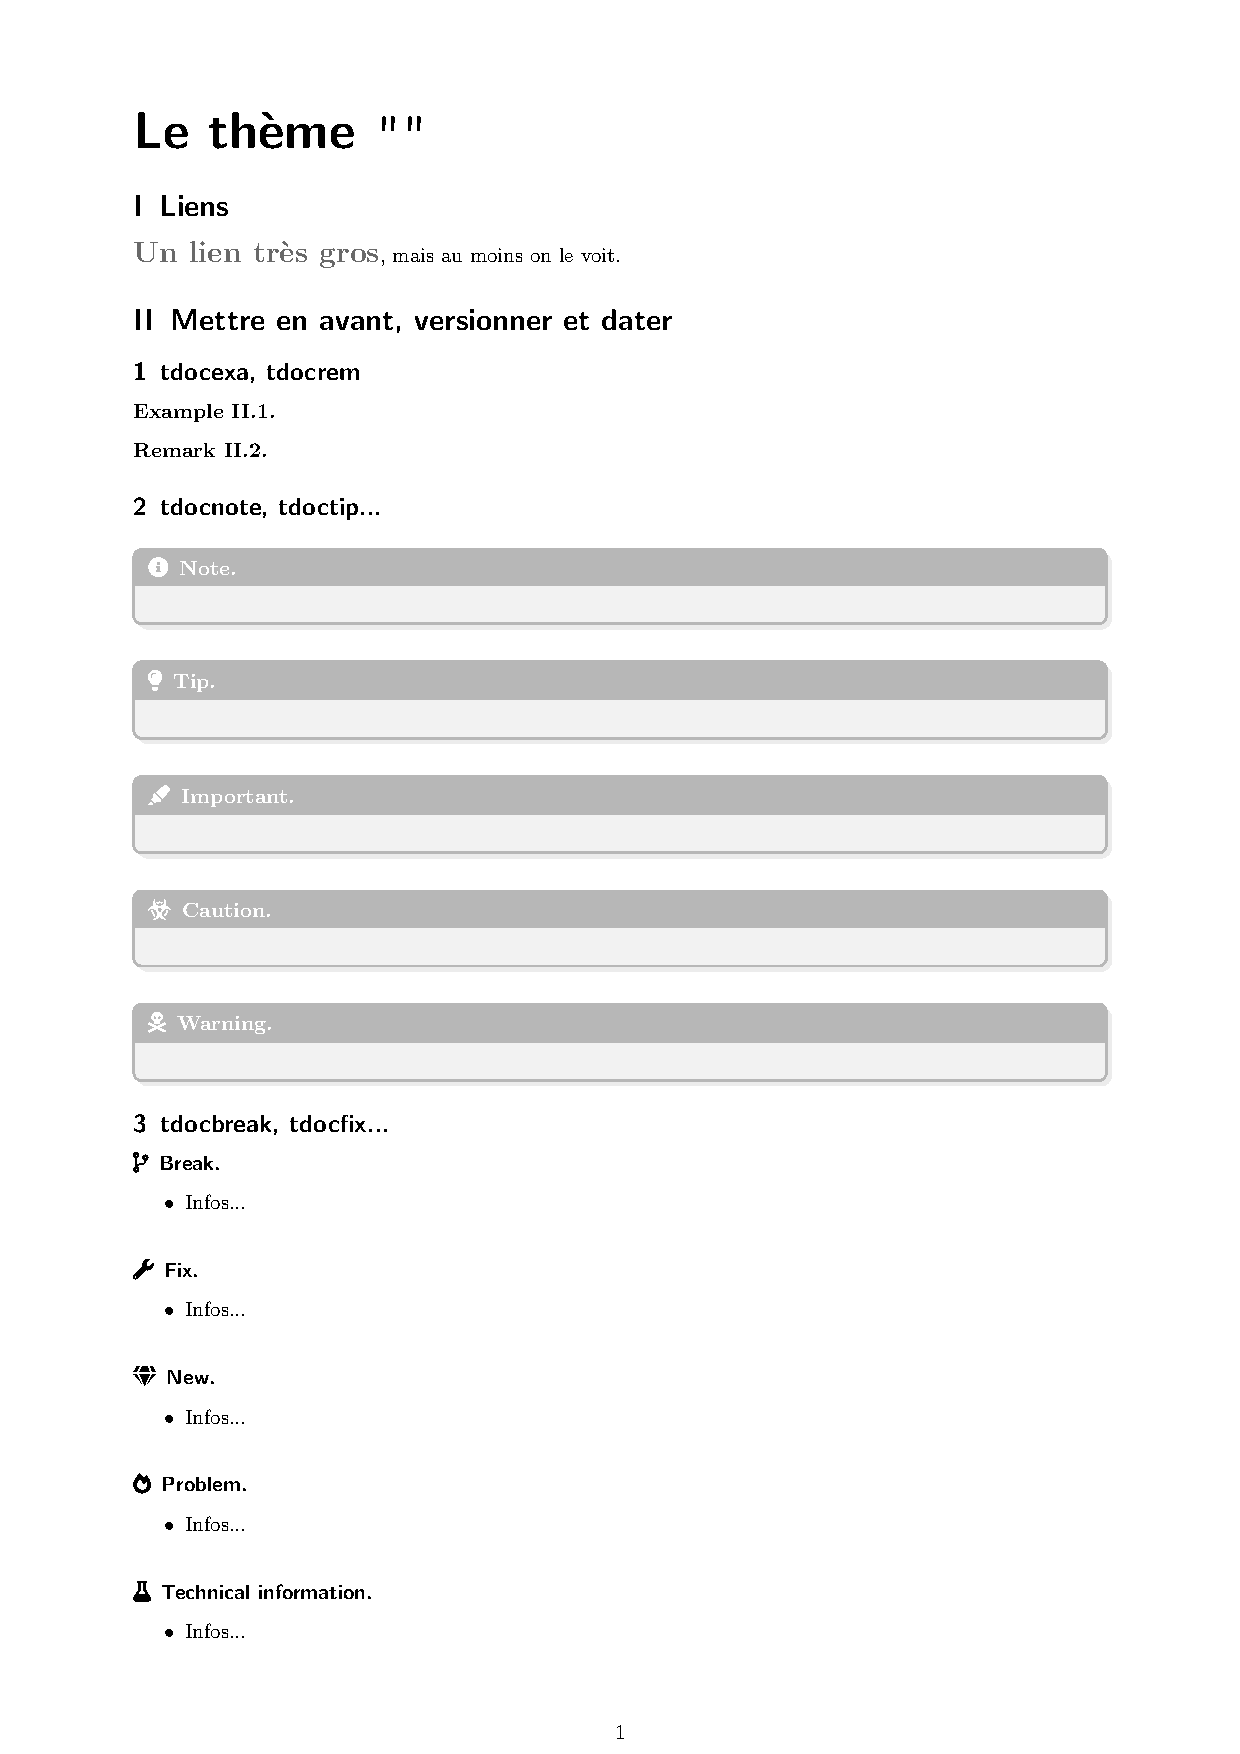
\includepdf{gallery-showcase-bw}

\includepdf{gallery-showcase-color}

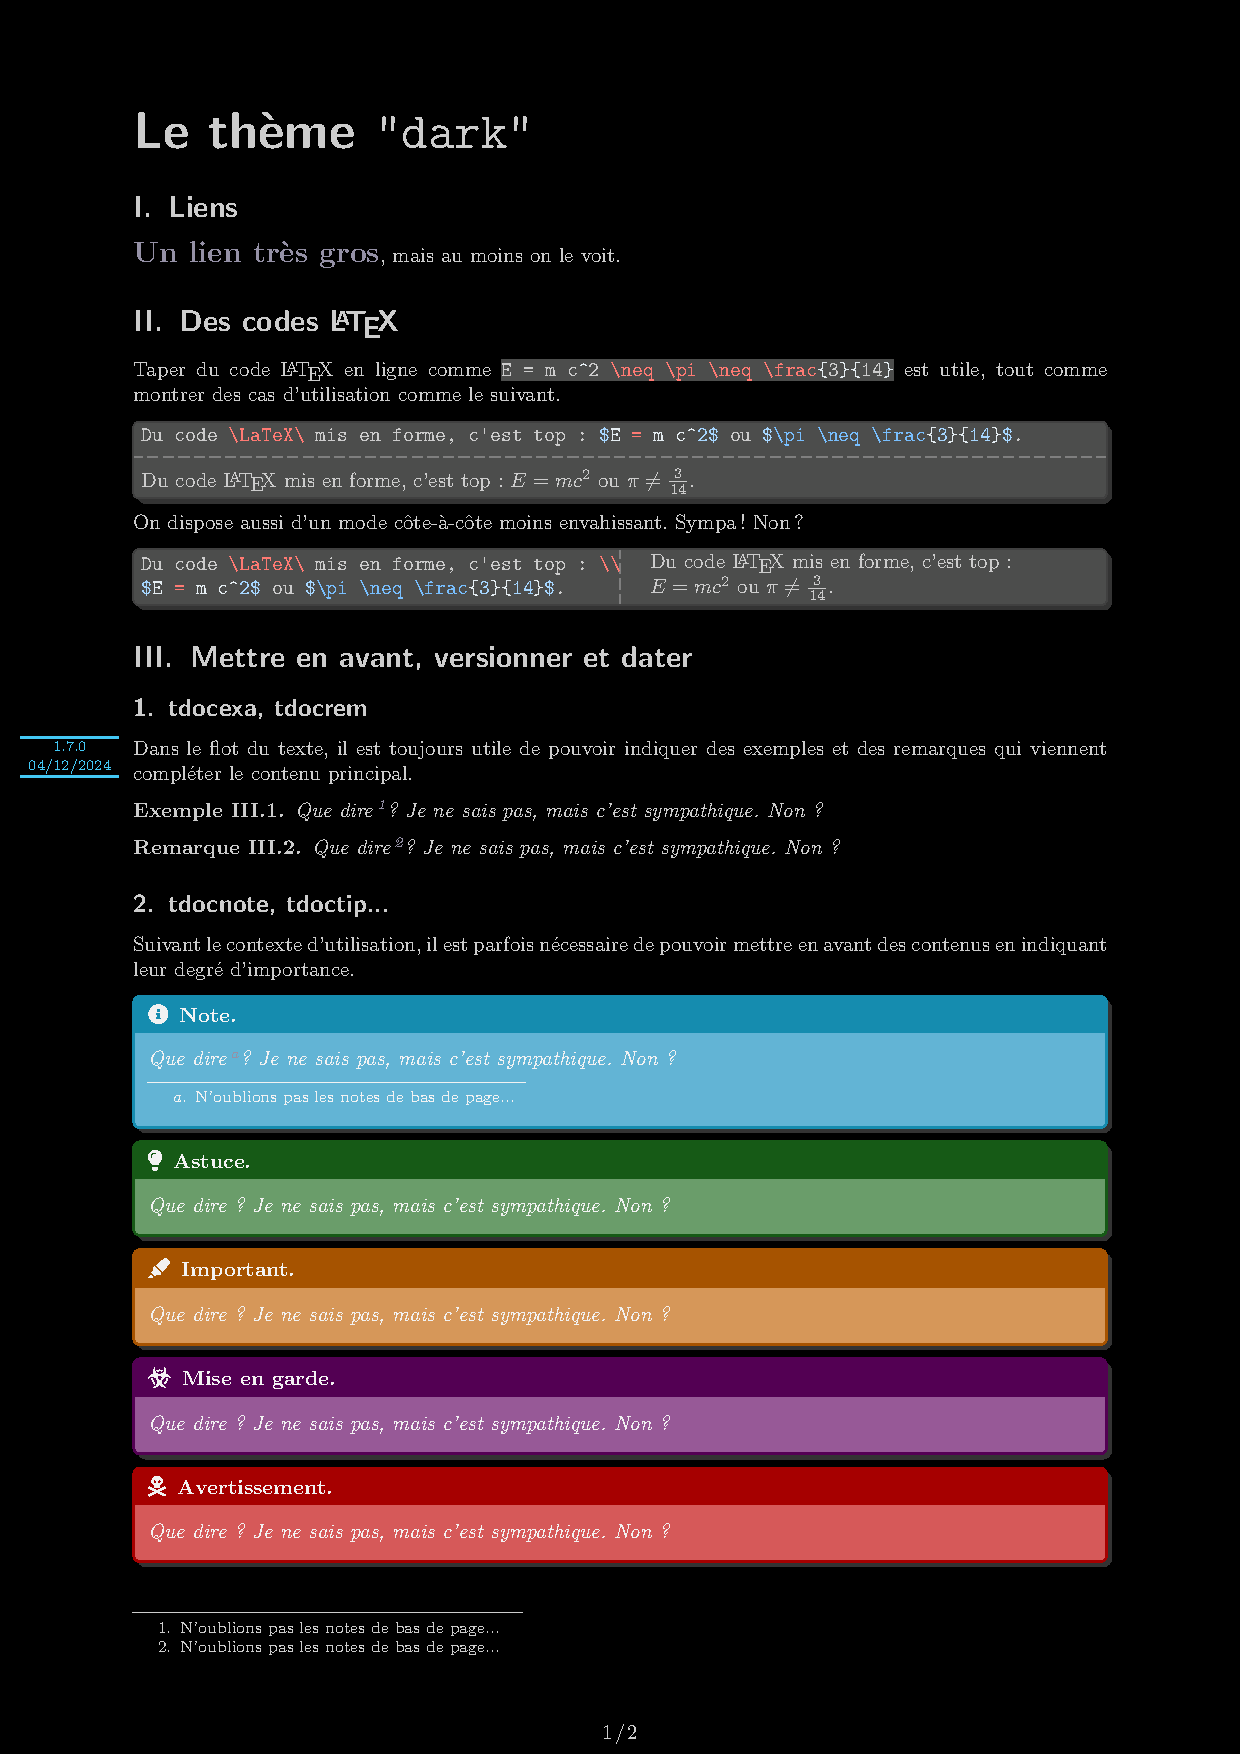
\includepdf{gallery-showcase-dark}

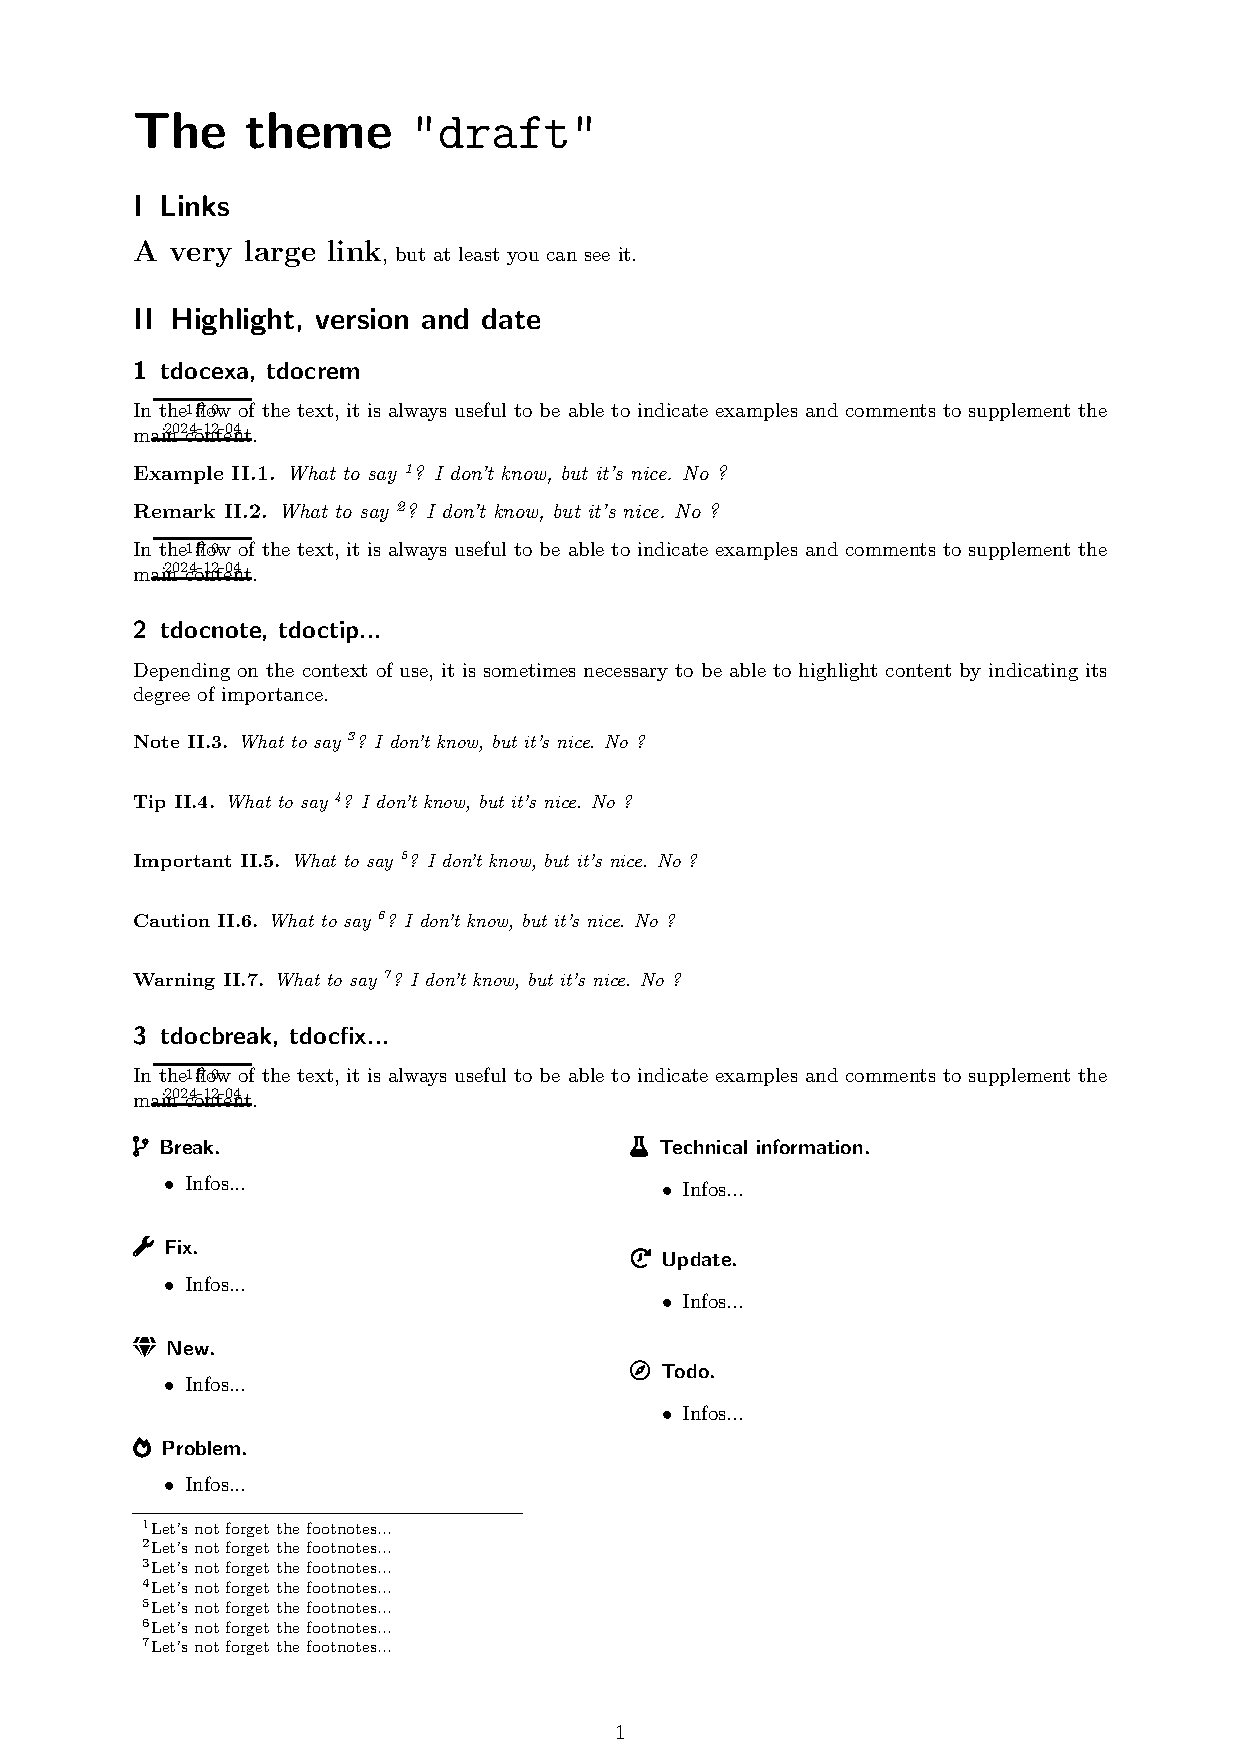
\includepdf{gallery-showcase-draft}

}

% --------------------------- %
% -- AT END DOCUMENT - END -- %
% --------------------------- %

\section{Mettre en avant du contenu}

\begin{tdocnote}
    Les environnements présentés dans cette section\,%
    \footnote{
        La mise en forme provient du package \tdocpack{keytheorems}.
    }
    ajoutent un court titre indiquant le type d'informations fournies.
    Ce court texte sera toujours traduit dans la langue repérée par la classe \thisproj.
\end{tdocnote}



\subsection{Du contenu dans le flot de la lecture}

\begin{tdocimp}
    Tous les environnements présentés dans cette section partagent le même compteur qui sera remis à zéro dès qu'une section de niveau au moins égale à une \tdoclatexin|\section| sera ouverte.
\end{tdocimp}



\subsubsection{Des exemples}

Des exemples numérotés, si besoin, s'indiquent via \tdocenv{tdocexa} qui propose un argument optionnel pour ajouter un mini-titre.
Voici deux usages possibles.

\tdoclatexinput<\tdoctcb{sbs}>{examples/admonitions/exa.tex}


\begin{tdoctip}
    Il peut parfois être utile de revenir à la ligne dès le début du contenu. Le code suivant montre comment faire (ce tour de passe-passe reste valable pour l'environnement \verb#tdocrem# présenté juste après). Noter au passage que la numérotation suit celle de l'exemple précédent comme souhaité.
\end{tdoctip}

\tdoclatexinput<\tdoctcb{sbs}>{examples/admonitions/exa-leavevmode.tex}


%\subsection{Du contenu dans le flot de la lecture}

\subsubsection{Des remarques}

Tout se passe via \tdocenv{tdocrem} avec un fonctionnement identique à l'environnement \tdocenv*{tdocexa} comme le montre l'exemple suivant.


\tdoclatexinput<\tdoctcb{sbs}>{examples/admonitions/rmk.tex}


\subsection{Du contenu tape-à-l'oeil}
\label{tutodoc-admonitions}

\begin{tdocnote}
    La mise en forme proposée ici est celle par défaut, mais d'autres sont possible en changeant de thème : voir la galerie de cas d'utilisation dans l'annexe page \pageref{tutodoc-theme-gallery}.
    Quant aux icônes, elles sont obtenues via le package \tdocpack{fontawesome5}, et la macro \tdocmacro{tdocicon} gère l'espacement vis-à-vis du texte.%
    \footnote{
        Par exemple,
        \tdoclatexin|\fbox{\tdocicon{\faBed}{Fatigué}}|
        produit\,
        \fbox{\tdocicon{\faBed}{Fatigué}}\,.
    }
\end{tdocnote}



\subsubsection{Une astuce}

L'environnement \tdocenv*{tdoctip} sert à donner des astuces. Voici comment l'employer.

\tdoclatexinput<\tdoctcb{sbs}, bottom = 3pt, top = 3pt>{examples/admonitions/tip.tex}


\smallskip


\begin{tdoctip}
    Quelque fois, un contenu mis en avant peut se réduire à une liste. Dans ce cas, la mise en forme peut être améliorée comme suit où nous utilisons l'option \tdoclatexin{wide} du package \tdocpack{enumitem} qui est importé par cette documentation.

    \tdoclatexinput<\tdoctcb{sbs}, bottom = 3pt, top = 3pt>{examples/admonitions/leavevmode-items.tex}
\end{tdoctip}


\foreach \sectitle/\desc/\filename in {
    {Note informative}/% <-- Translate me!
    {L'environnement \tdocenv*{tdocnote} sert à mettre en avant des informations utiles. Voici comment l'utiliser.}/% <-- Translate me!
    note,
    %
    {Un truc important}/% <-- Translate me!
    {L'environnement \tdocenv*{tdocimp} permet d'indiquer quelque chose d'important mais sans danger.}/% <-- Translate me!
    important,
    %
    {Avertir d'un point très délicat}/% <-- Translate me!
    {L'environnement \tdocenv*{tdoccaut} sert à indiquer un point délicat à  l'utilisateur. Voici comment l'employer.}/%<-- Translate me!
    caution,
    %
    {Avertir d'un danger}/% <-- Translate me!
    {L'environnement \tdocenv*{tdocwarn} sert à avertir l'utilisateur d'un piège à éviter. Voici comment l'employer.}/% <-- Translate me!
    warn%
} {
    \subsubsection{\sectitle}

    \desc

    \tdoclatexinput<\tdoctcb{sbs}, bottom = 3pt, top = 3pt>{examples/admonitions/\filename.tex}
}


\section{Indiquer des packages, des classes, des macros ou des environnements}

Voici ce qu'il est possible de taper de façon sémantique.


\begin{tdoclatex}<\tdoctcb{sbs}>
\tdoccls{maclasse} sert à...           \\
\tdocpack{monpackage} est pour...      \\
\tdocmacro{unemacro} permet de...      \\
\tdocenv{env} produit...               \\
\tdocenv[{[opt1]<opt2>}]{env}          \\
Juste \tdocenv*{env}...                \\
Enfin \tdocenv*[{[opt1]<opt2>}]{env}...
      % Pour les copier-coller.
\end{tdoclatex}


\begin{tdocrem}
    Contrairement à \tdocmacro{tdoclatexin}, les macros \tdocmacro{tdocenv} et \tdocmacro{tdocenv*} ne colorent pas le texte produit.
    De plus, \tdoclatexin{\tdocenv{monenv}} produit \tdocenv{monenv} avec des espaces afin d'autoriser des retours à la ligne si besoin.
\end{tdocrem}


\begin{tdocwarn}
    L'argument optionnel de la macro \tdocmacro{tdocenv} est copié-collé\,%
    \footnote{
        Se souvenir que tout est possible ou presque dorénavant.
    }
    lors du rendu. Ceci peut donc parfois nécessiter d'utiliser des accolades protectrices comme dans l'exemple ci-dessus.
\end{tdocwarn}



\section{Origine d'un préfixe ou d'un suffixe}

Pour expliquer les noms retenus, rien de tel que d'indiquer et expliciter les courts préfixes et suffixes employés. Ceci se fait facilement comme suit.


\begin{tdoclatex}<\tdoctcb{sbs}>
\tdocpre{sup} est relatif à...    \\
\tdocprewhy{sup.erbe} signifie... \\
\emph{\tdocprewhy{sup.er} pour...}
\end{tdoclatex}


\begin{tdocrem}
    Le choix du point pour scinder un mot permet d'utiliser des mots avec un tiret comme dans \tdoclatexin+\tdocprewhy{ca.sse-brique}+ qui donne \tdocprewhy{ca.sse-brique}.
\end{tdocrem}


\section{Un rendu en situation réelle}
\label{tutodoc-showcase}

Il est parfois utile d'obtenir directement le rendu d'un code dans la documentation. Ceci nécessite que ce type de rendu soit dissociable du texte donnant des explications.



\subsection{Un rendu minimaliste par défaut}

\begin{tdocexa}[Avec les textes par défaut]
    Il peut être utile de montrer un rendu réel directement dans un document.%
    \footnote{
        Typiquement lorsque l'on fait une démo.
    }
    Ceci se tape via \tdocenv{tdocshowcase} comme suit.

    \tdoclatexshow[explain = {On obtient alors le rendu suivant qui est juste la combinaison d'un faible espacement vertical et d'une simple importation.}]%
                  {examples/showcase/default.tex}
\end{tdocexa}


\begin{tdocrem}
    La section \ref{tutodoc-listing-latexshow} page \pageref{tutodoc-listing-latexshow} explique comment obtenir, via la macro \tdocmacro{tdoclatexshow}, un code suivi de son rendu réel comme dans l'exemple précédent.
\end{tdocrem}


\begin{tdocwarn}
    Avec les paramètres par défaut, si le code à formater commence par un crochet ouvrant, utilisez l'une des astuces suivantes.

    \tdoclatexshow[explain = {Ceci produira ce qui suit.}]%{
    		      {examples/showcase/hook.tex}
\end{tdocwarn}


\subsection{Avec des lignes cadrantes}

Pour rendre plus visible le code \LaTeX\ mis en forme de façon sombre, on peut faire appel au style \tdoclatexin{rule} comme dans les exemple suivants.


\begin{tdocexa}
	L'option \tdoclatexin{style=rule} permet d'obtenir ce qui suit ce qui suit où les textes ajoutés automatiquement s'adapteront à la langue repéré par \thisproj.

	\documentclass{tutodoc}

\usepackage[utf8]{inputenc}
\usepackage[T1]{fontenc}

\usepackage[french]{babel, varioref}

\usepackage{enumitem}
\frenchsetup{StandardItemLabels=true}

\usepackage{tabularray}

\usepackage[lang = french]{tutodoc}



\begin{document}

\subsection{Avec des lignes cadrantes}

Pour rendre plus visible le code \LaTeX\ mis en forme de façon sombre, on peut faire appel au style \tdoclatexin{rule} comme dans les exemple suivants.


\begin{tdocexa}
	L'option \tdoclatexin{style=rule} permet d'obtenir ce qui suit ce qui suit où les textes ajoutés automatiquement s'adapteront à la langue repéré par \thisproj.

	\documentclass{tutodoc}

\usepackage[utf8]{inputenc}
\usepackage[T1]{fontenc}

\usepackage[french]{babel, varioref}

\usepackage{enumitem}
\frenchsetup{StandardItemLabels=true}

\usepackage{tabularray}

\usepackage[lang = french]{tutodoc}



\begin{document}

\subsection{Avec des lignes cadrantes}

Pour rendre plus visible le code \LaTeX\ mis en forme de façon sombre, on peut faire appel au style \tdoclatexin{rule} comme dans les exemple suivants.


\begin{tdocexa}
	L'option \tdoclatexin{style=rule} permet d'obtenir ce qui suit ce qui suit où les textes ajoutés automatiquement s'adapteront à la langue repéré par \thisproj.

	\documentclass{tutodoc}

\input{../preamble.cfg.tex}


\begin{document}

\subsection{Avec des lignes cadrantes}

Pour rendre plus visible le code \LaTeX\ mis en forme de façon sombre, on peut faire appel au style \tdoclatexin{rule} comme dans les exemple suivants.


\begin{tdocexa}
	L'option \tdoclatexin{style=rule} permet d'obtenir ce qui suit ce qui suit où les textes ajoutés automatiquement s'adapteront à la langue repéré par \thisproj.

	\input{examples/showcase/rule.tex}
\end{tdocexa}


\begin{tdocexa}[Du texte et des couleurs modifiables]
	On peut obtenir facilement l'horreur suivante.

	\input{examples/showcase/rule-custom.tex}
	
	Voici le code qui a été employé.%
	\footnote{
		La section suivante va normaliser le choix, a priori étrange, de \tdoclatexin{col-stripe} au lieu de \tdoclatexin{col-rule}\,.
	}

	\tdoclatexinput<\tdoctcb{code}>{examples/showcase/rule-custom.tex}
\end{tdocexa}


\begin{tdocnote}
    Dans l'exemple précédent, le texte utilise bien l'orange assombri proposé. Par contre, le rouge sert de base pour obtenir les couleurs utilisées pour la bande : les transformations utilisées dépendent du thème choisi.%
    \footnote{
        Par exemple, les thèmes \tdoclatexin{bw} et \tdoclatexin{draft} ne tiennent pas compte de la clé \tdoclatexin{col-stripe} !
    }
    %
    Il faut également savoir qu'en coulisse, la macro \tdocmacro{tdocruler} est employée.

    \begin{tdoclatex}<\tdoctcb{std}>
\tdocruler[red]{Un pseudo-titre décoré}
    \end{tdoclatex}
\end{tdocnote}

\end{document}

\end{tdocexa}


\begin{tdocexa}[Du texte et des couleurs modifiables]
	On peut obtenir facilement l'horreur suivante.

	\begin{tdocshowcase}[style      = rule,
                     col-stripe = red,
                     col-text   = orange!75!black,
                     before     = Mon début,
                     after      = Ma fin à moi]
    Bla, bla, bla, bla, bla, bla, bla, bla, bla, bla, bla, bla, bla...
\end{tdocshowcase}

	
	Voici le code qui a été employé.%
	\footnote{
		La section suivante va normaliser le choix, a priori étrange, de \tdoclatexin{col-stripe} au lieu de \tdoclatexin{col-rule}\,.
	}

	\tdoclatexinput<\tdoctcb{code}>{examples/showcase/rule-custom.tex}
\end{tdocexa}


\begin{tdocnote}
    Dans l'exemple précédent, le texte utilise bien l'orange assombri proposé. Par contre, le rouge sert de base pour obtenir les couleurs utilisées pour la bande : les transformations utilisées dépendent du thème choisi.%
    \footnote{
        Par exemple, les thèmes \tdoclatexin{bw} et \tdoclatexin{draft} ne tiennent pas compte de la clé \tdoclatexin{col-stripe} !
    }
    %
    Il faut également savoir qu'en coulisse, la macro \tdocmacro{tdocruler} est employée.

    \begin{tdoclatex}<\tdoctcb{std}>
\tdocruler[red]{Un pseudo-titre décoré}
    \end{tdoclatex}
\end{tdocnote}

\end{document}

\end{tdocexa}


\begin{tdocexa}[Du texte et des couleurs modifiables]
	On peut obtenir facilement l'horreur suivante.

	\begin{tdocshowcase}[style      = rule,
                     col-stripe = red,
                     col-text   = orange!75!black,
                     before     = Mon début,
                     after      = Ma fin à moi]
    Bla, bla, bla, bla, bla, bla, bla, bla, bla, bla, bla, bla, bla...
\end{tdocshowcase}

	
	Voici le code qui a été employé.%
	\footnote{
		La section suivante va normaliser le choix, a priori étrange, de \tdoclatexin{col-stripe} au lieu de \tdoclatexin{col-rule}\,.
	}

	\tdoclatexinput<\tdoctcb{code}>{examples/showcase/rule-custom.tex}
\end{tdocexa}


\begin{tdocnote}
    Dans l'exemple précédent, le texte utilise bien l'orange assombri proposé. Par contre, le rouge sert de base pour obtenir les couleurs utilisées pour la bande : les transformations utilisées dépendent du thème choisi.%
    \footnote{
        Par exemple, les thèmes \tdoclatexin{bw} et \tdoclatexin{draft} ne tiennent pas compte de la clé \tdoclatexin{col-stripe} !
    }
    %
    Il faut également savoir qu'en coulisse, la macro \tdocmacro{tdocruler} est employée.

    \begin{tdoclatex}<\tdoctcb{std}>
\tdocruler[red]{Un pseudo-titre décoré}
    \end{tdoclatex}
\end{tdocnote}

\end{document}

\end{tdocexa}


\begin{tdocexa}[Du texte et des couleurs modifiables]
	On peut obtenir facilement l'horreur suivante.

	\begin{tdocshowcase}[style      = rule,
                     col-stripe = red,
                     col-text   = orange!75!black,
                     before     = Mon début,
                     after      = Ma fin à moi]
    Bla, bla, bla, bla, bla, bla, bla, bla, bla, bla, bla, bla, bla...
\end{tdocshowcase}

	
	Voici le code qui a été employé.%
	\footnote{
		La section suivante va normaliser le choix, a priori étrange, de \tdoclatexin{col-stripe} au lieu de \tdoclatexin{col-rule}\,.
	}

	\tdoclatexinput<\tdoctcb{code}>{examples/showcase/rule-custom.tex}
\end{tdocexa}


\begin{tdocnote}
    Dans l'exemple précédent, le texte utilise bien l'orange assombri proposé. Par contre, le rouge sert de base pour obtenir les couleurs utilisées pour la bande : les transformations utilisées dépendent du thème choisi.%
    \footnote{
        Par exemple, les thèmes \tdoclatexin{bw} et \tdoclatexin{draft} ne tiennent pas compte de la clé \tdoclatexin{col-stripe} !
    }
    %
    Il faut également savoir qu'en coulisse, la macro \tdocmacro{tdocruler} est employée.

    \begin{tdoclatex}<\tdoctcb{std}>
\tdocruler[red]{Un pseudo-titre décoré}
    \end{tdoclatex}
\end{tdocnote}


\subsection{Avec une bande colorée}

Il est des situations où l'on doit pouvoir clairement identifier un exemple de code \LaTeX\ mis en forme. Ceci est faisable comme le montrent les exemples suivants.%
\footnote{
    En coulisse, les bandes sont créées sans effort grâce au package \tdocpack{clrstrip}.
}


\begin{tdocexa}
	L'option \tdoclatexin{style=stripe} fournit ce qui suit.

	\documentclass[10pt, a4paper]{article}

\usepackage[utf8]{inputenc}
\usepackage[T1]{fontenc}

\usepackage[french]{babel, varioref}

\usepackage{enumitem}
\frenchsetup{StandardItemLabels=true}

\usepackage{tabularray}

\usepackage[lang = french]{tutodoc}


\usepackage[lang = french]{../main/main}
\usepackage{../macroenv/macroenv}
\usepackage{../listing/listing}
\usepackage{../focus/focus}

% TESTING LOCAL IMPLEMENTATION %

\usepackage{showcase}


\begin{document}

\section{Un rendu en situation réelle} \label{tdoc-showcase}

Il est parfois utile d'obtenir directement le rendu d'un code dans la documentation. Ceci nécessite que ce type de rendu soit dissociable du texte donnant des explications.


% ------------------ %


\subsection{Avec une bande colorée}

\begin{tdocexa}[Avec les textes par défaut]
    Il peut être utile de montrer un rendu réel directement dans un document
    \footnote{
        Typiquement lorsque l'on fait une démo.
    }.
    Ceci se tape via \tdocenv{tdocshowcase} comme suit.

    \tdoclatexinput[code]{examples/showcase/default.tex}

    On obtient alors le rendu suivant
    \footnote{
        En coulisse, la bande est créée sans effort grâce au package \tdocpack{clrstrip}.
    }.

    \medskip

    \begin{bdocshowcase}
    \bfseries Un peu de code \LaTeX.

    \bigskip

    \emph{\large Fin de l'affreuse démo.}
\end{bdocshowcase}
\end{tdocexa}


\begin{tdocrem}
    Voir la section \ref{tdoc-latexshow} page \pageref{tdoc-latexshow} pour obtenir facilement un code suivi de son rendu réel comme dans l'exemple précédent.
\end{tdocrem}


\begin{tdocnote}
    Les textes explicatifs s'adaptent à la langue choisie lors du chargement de \tdocpack{tutodoc}.
\end{tdocnote}


% ------------------ %


\begin{tdocexa}[Changer la couleur et/ou les textes par défaut]
    \leavevmode

    \tdoclatexinput[code]{examples/showcase/customized.tex}

    Ceci produira ce qui suit.

    \medskip

    
\begin{bdocshowcase}[before = Mon début,   
                     after  = Ma fin à moi,
                     color  = red]
    Bla, bla, bla, bla, bla, bla, bla, bla, bla, bla, bla, bla, bla...
\end{bdocshowcase}
\end{tdocexa}


\begin{tdocnote}
    Vous avez sûrement noté que l'on n'obtient pas un rouge pur : en coulisse les macros développables \tdocmacro{tdocbackcolor} et \tdocmacro{tdocdarkcolor} sont utilisées pour créer celles du fond et des titres respectivement à partir de la couleur proposée à \tdocenv{tdocshowcase}.
    Ces macros à un seul argument, la couleur choisie, admettent les codes suivants.

    \begin{tdoclatex}[code]
\NewExpandableDocumentCommand{\tdocbackcolor}{m}{#1!5}
\NewExpandableDocumentCommand{\tdocdarkcolor}{m}{#1!50!black}
    \end{tdoclatex}
\end{tdocnote}


% ------------------ %


\begin{tdocwarn}
    Avec les réglages par défaut, si le code \LaTeX\ à mettre en forme commence par un crochet ouvrant, il faudra indiquer explicitement une option vide comme dans l'exemple suivant.

    \tdoclatexinput[code]{examples/showcase/hook.tex}

    Ceci produira ce qui suit.

    \medskip

    \begin{tdocshowcase}
    \string[Cela fonctionne...]
\end{tdocshowcase}

\end{tdocwarn}


\begin{tdocnote}
    Il faut savoir qu'en coulisse la macro \tdocmacro{tdocruler} est utilisée.

    \begin{tdoclatex}[std]
        \tdocruler{Un pseudo-titre décoré}{red}
    \end{tdoclatex}
\end{tdocnote}

\end{document}

\end{tdocexa}


\begin{tdocexa}[Du texte et des couleurs modifiables]
	On peut produire facilement une belle horreur comme celle qui arrive.

	\begin{tdocshowcase}[style      = stripe,
                     col-stripe = green,
                     col-text   = purple,
                     before     = Mon début,
                     after      = Ma fin à moi]
    Bla, bla, bla, bla, bla, bla, bla, bla, bla, bla, bla, bla, bla...
\end{tdocshowcase}

	
	Voici le code qui a été employé.%
	\footnote{
		On comprend maintenant le choix de \tdoclatexin{col-stripe} au lieu de \tdoclatexin{col-rule}\,.
	}

	\tdoclatexinput<\tdoctcb{code}>{examples/showcase/stripe-custom.tex}
\end{tdocexa}


\subsection{En important le code \LaTeX}

Pour obtenir des rendus en important le code depuis un fichier externe, au lieu de le taper, il suffit d'employer la macro \tdocmacro{tdocshowcaseinput} dont l'option reprend la syntaxe de celle de l'environnement \tdocenv*{tdocshowcase} et l'argument obligatoire correspond au chemin du fichier. Voici des exemples d'utilisation de \tdoclatexin+\tdocshowcaseinput{external.tex}+ avec ou sans option.


\foreach \exatitle/\option in {
    {Sans option}/% <-- Translate me!
    {},
    {Juste les lignes cadrantes}/% <-- Translate me!
    {style=rule},
    {Une bande colorée}/% <-- Translate me!
    {style=stripe, col-stripe=red, col-text=LightCoral}%
}{
	\begin{tdocexa}[\exatitle]
		\expandafter\IfBlankTF\expandafter{\option}{
			Voici le contenu édifiant de l'exemple choisi.
			
	    	\tdocshowcaseinput{examples/showcase/external.tex}
		}{
	    	L'option \expandafter\tdoclatexin\expandafter{\option} fournit ce qui suit.
		
			\smallskip
			\expandafter\tdocshowcaseinput\expandafter[\option]{examples/showcase/external.tex}
		}
	\end{tdocexa}
}


\section{Cas d'utilisation en \LaTeX}
\label{tutodoc-listing-latex}

Documenter un package ou une classe se fait efficacement via des cas d'utilisation montrant à la fois du code et le résultat correspondant.%
\footnote{
    La mise en forme des codes se fait via les packages \tdocpack{minted} et  \tdocpack{tcolorbox}.
}



\subsection{Codes \tdocquote{en ligne}}
\label{tutodoc-listing-latex-inline}

\begin{tdocexa}[Usage standard]
    La macro \tdocmacro{tdoclatexin}\,%
    \footnote{
        Le nom de la macro \tdocmacro{tdoclatexin} vient de \tdocquote{\tdocprewhy{in.line} \LaTeX} soit \tdocinEN{\LaTeX\ en ligne}.
    }
    permet de taper du code en ligne via un usage similaire à \tdocmacro{verb}, ou bien comme une macro standard (voir la gestion des accolades dans le dernier cas ci-dessous).
    Voici des exemples d'utilisation.%
    \footnote{
    	Une couleur de fond est volontairement utilisée pour subtilement faire ressortir les codes \tdoclatexin{\LaTeX}\,.
    }

    \begin{tdoclatex}<\tdoctcb{sbs}>
1: \tdoclatexin|$a^b = c$|               \\
2: \tdoclatexin+\tdoclatexin|$a^b = c$|+ \\
3: \tdoclatexin{\tdoclatexin{$a^b = c$}}
	\end{tdoclatex}
\end{tdocexa}


\begin{tdocexa}[Des options possibles]
    Comme la macro \tdocmacro{tdoclatexin} s'appuie sur \tdocpack{minted}, on peut utiliser toutes les options prises en compte par \tdocpack{minted}.
    Voici des exemples d'utilisation.

    \begin{tdoclatex}<\tdoctcb{sbs}>
1: \tdoclatexin{$a^b = c$}             \\
2: \tdoclatexin[style = bw]{$a^b = c$} \\
3: \tdoclatexin[style = igor,
                showspaces]{$a^b = c$}
	\end{tdoclatex}
\end{tdocexa}


\begin{tdocnote}
    La macro \tdocmacro{tdoclatexin} est utilisable dans une note de pied de page : voir ci-dessous.%
    \footnote{
        \tdoclatexin+$minted = TOP$+ a été tapé \tdoclatexin|\tdoclatexin+$minted = TOP$+| dans cette note de bas de page.
    }
\end{tdocnote}



\subsection{Codes tapés directement}

\begin{tdocexa}[Face à face]
    Afficher un code et son rendu côte à côte se fait comme suit où la macro \tdocmacro{tdoctcb} permet de juste taper \tdoclatexin{\tdoctcb{sbs}} au lieu de \tdoclatexin{listing side text} (\tdoclatexin#sbs# est pour \tdocquote{\tdocprewhy{s.ide} \tdocprewhy{b.y} \tdocprewhy{s.ide}} soit \tdocinEN{côte à côte}, tandis que \tdoclatexin#tcb# est l'abréviation standard de \texttt{tcolorbox}). Bien noter l'emploi de chevrons, et non de crochets (nous revenons sur ceci un plus bas).

    \tdoclatexshow{examples/listing-latex/ABC.tex}
\end{tdocexa}


\begin{tdocexa}[À la suite]
    \tdocenv{tdoclatex} produit le résultat suivant (ce réglage par défaut s'obtient aussi via l'emploi de \tdoclatexin#\tdoctcb{std}#).%
    \footnote{
        \tdoclatexin{std} fait référence au comportement \tdocquote{standard} de \tdocpack{tcolorbox} vis à vis de la librairie \tdocpack{minted}.
    }

    \begin{tdoclatex}
$A = B + C$
    \end{tdoclatex}
\end{tdocexa}


\begin{tdocexa}[Juste le code]
    Via \tdoclatexin#\tdoctcb{code}#, on aura juste le code comme ci-après.

    \begin{tdoclatex}<\tdoctcb{code}>
$A = B + C$
    \end{tdoclatex}
\end{tdocexa}


\begin{tdocexa}[Personnaliser]
	L'environnement \tdocenv*{tdoclatex} accepte deux types d'argument optionnel.
	%
	\begin{enumerate}
		\item Entre de classiques crochets, on peut employer toute option prise en compte par \tdocpack{minted}.

        \item Entre des chevrons, on peut employer toute option prise en compte par les environnements obtenus via \tdocpack{tcolorbox}.
	\end{enumerate}

	Par exemple, on peut faire les modifications suivantes si besoin.%
	\footnote{
		Cette documentation utilise les options entre chevrons pour obtenir des rendus corrects de codes \LaTeX\ produisant des cadres ombrés : voir la section \ref{tutodoc-admonitions} page \pageref{tutodoc-admonitions}.
	}

    \tdoclatexshow{examples/listing-latex/ABC-custom.tex}
\end{tdocexa}

\medskip

\begin{tdocwarn}
    Pour obtenir la mise en forme par défaut d'un code commençant par un crochet, ou un chevron, il faudra bidouiller un peu comme ci-dessous.
    \tdoclatexshow{examples/listing-latex/strange.tex}

    \smallskip

    Une autre méthode consiste à utiliser la primitive \tdocmacro{string} comme ci-après.
    \tdoclatexshow{examples/listing-latex/strange-bis.tex}
    \end{tdocwarn}


\subsection{Codes importés}

Pour les codes suivants, on considère un fichier de chemin relatif \verb+examples-listing-xyz.tex+, et ayant le contenu suivant.


\tdoclatexinput<\tdoctcb{code}>{examples-listing-latex-xyz.tex}


\medskip


La macro \tdocmacro{tdoclatexinput}, présentée ci-dessous, attend le chemin d'un fichier et propose le même système d'options entre crochets, ou entre chevrons, que l'environnement \tdocenv*{tdoclatex}.


\begin{tdocexa}[Face à face]
    \leavevmode

    \begin{tdoclatex}<\tdoctcb{code}>
\tdoclatexinput<\tdoctcb{sbs}>{examples-listing-latex-xyz.tex}
    \end{tdoclatex}

    Ceci produit la mise en forme suivante.

    \tdoclatexinput<\tdoctcb{sbs}>{examples-listing-latex-xyz.tex}
\end{tdocexa}


\begin{tdocexa}[À la suite]
    \leavevmode

    \begin{tdoclatex}<\tdoctcb{code}>
\tdoclatexinput{examples-listing-latex-xyz.tex}
    \end{tdoclatex}

    Ceci produit la mise en forme suivante qui correspond aussi à l'option \tdoclatexin#\tdoctcb{std}#\,.

    \tdoclatexinput{examples-listing-latex-xyz.tex}
\end{tdocexa}


\begin{tdocexa}[Juste le code]
    \leavevmode

    \begin{tdoclatex}<\tdoctcb{code}>
\tdoclatexinput<\tdoctcb{code}>{examples-listing-latex-xyz.tex}
    \end{tdoclatex}

    Ceci produit la mise en forme suivante.

    \tdoclatexinput<\tdoctcb{code}>{examples-listing-latex-xyz.tex}
\end{tdocexa}


\begin{tdocexa}[Personnaliser]
    \leavevmode

    \begin{tdoclatex}<\tdoctcb{code}>
\tdoclatexinput[style=igor, showspaces]<\tdoctcb{code}>{examples-listing-latex-xyz.tex}
    \end{tdoclatex}

    Ceci produit la mise en forme suivante.

	\tdoclatexinput[style = igor, showspaces]<\tdoctcb{code}>{examples-listing-latex-xyz.tex}
\end{tdocexa}



\subsection{Codes importés et mis en situation}
\label{tutodoc-listing-latexshow}

\begin{tdocnote}
    Les textes par défaut de la macro \tdocmacro{tdoclatexshow} tiennent compte de la langue détectée par \thisproj.
\end{tdocnote}


\begin{tdocexa}[Mise en situation]
    \tdoclatexin+\tdoclatexshow{examples-listing-xyz.tex}+ produit ce qui suit.

    \smallskip
    
    \tdoclatexshow{examples-listing-latex-xyz.tex}
\end{tdocexa}


\begin{tdocexa}[Changer le texte explicatif]
    Via la clé \tdoclatexin|explain|, on peut utiliser un texte personnalisé. Ainsi, \tdoclatexin|\tdoclatexshow[explain = Voici le rendu réel.]{examples-listing-xyz.tex}| produira ce qui suit.

    \smallskip

    \tdoclatexshow[explain = Voici le rendu réel.]{examples-listing-latex-xyz.tex}
\end{tdocexa}


\begin{tdocexa}[Les options disponibles]
    En plus du texte explicatif, il est aussi possible d'utiliser toutes les options de l'environnement \tdocenv*{tdocshowcase}, voir la section \ref{tutodoc-showcase} page \pageref{tutodoc-showcase}.
    Voici un exemple illustrant ceci.

    \medskip

    \tdoclatexinput<\tdoctcb{code}>{examples/listing-latex/latexshow-options.tex}

    \smallskip

    Ceci va produire ce qui suit.

    \smallskip

    \tdoclatexshow[style      = stripe,
               col-stripe = orange,
               col-text   = blue!70!black,
               before     = Rendu ci-après.,
               explain    = Ce qui vient est coloré...,
               after      = Rendu fini.,]
               {examples/listing-latex/xyz.tex}

\end{tdocexa}


\section{Présenter du code informatique}

Certains packages proposent des outils utilisables via le langage \lua\ depuis un document \LaTeX.%
\footnote{
	Pour les mathématiques, on peut citer \tdocpack{luacas} et \tdocpack{tkz-elements}.
}
Pour ce type de projet, il est utile de pouvoir présenter des lignes de code \lua\ ; \thisproj\ permet de faire cela aisément, et bien plus.%
\footnote{
    La mise en forme des codes étant faite via les packages \tdocpack{minted} et \tdocpack{tcolorbox}, les macros et les environnements présentés dans cette section permettent la mise en forme de codes dans tous les langages supportés par \pygmentsREF, un projet \python\ utilisé en coulisse par \tdocpack{minted}.
}


\begin{tdoccaut}
	Les outils de cette section permettent aussi de présenter du code \LaTeX, mais il ne faut pas les utiliser pour de simples cas d'utilisation.
	Les macros et les environnements présentées juste après servent à étudier du code, et non juste à l'employer : se reporter à la section \ref{tutodoc-listing-latex} page \pageref{tutodoc-listing-latex} pour employer les bons outils pour mettre en forme de simples cas d'utilisation.
\end{tdoccaut}



\subsection{Codes \tdocquote{en ligne}}

ZZZ


\tdocodein{py}{print("Hello!")}


\tdocodeinput{py}{examples-listing-full-hello-you.py}


\subsection{Codes importés}

\tdocodeinput{lua}{examples-listing-full-hello-you.lua}

\tdocodeinput{java}{examples-listing-full-hello-you.java}

\tdocodeinput{tex}{examples-listing-full-hello-you.tex}

\tdocodeinput{pl}{examples-listing-full-hello-you.pl}

\tdocodeinput{python}{examples-listing-full-hello-you.py}

\tdocodeinput{brainfuck}{examples-listing-full-hello-world.b}


\section{Indiquer les changements}
\label{tutodoc-changes}

Afin de faciliter le suivi d'un projet, il est indispensable de fournir un historique indiquant les changements effectués lors de la publication d'une nouvelle version.



\subsection{À quel moment ?}
\label{tutodoc-changes-when}

On peut au choix dater quelque chose, ou bien le versionner, dans ce second cas le numéro de version pourra éventuellement être daté.


\begin{tdocexa}[Dater des nouveautés]
    La macro \tdocmacro{tdocdate} permet d'indiquer une date dans la marge comme dans l'exemple suivant.

    \tdoclatexshow{examples/version-n-change/dating.tex}
\end{tdocexa}


\begin{tdocexa}[Versionner des nouveautés en les datant événtuellement]
    Associer un numéro de version à une nouveauté se fait via la macro \tdocmacro{tdocversion}, la couleur et la date étant des arguments optionnels.

    \tdoclatexshow{examples/version-n-change/versioning.tex}
\end{tdocexa}


\begin{tdocexa}[Attention avec les titres de paragraphe]
	L'exemple suivant montre qu'il faut placer une dates et/ou une version juste après un titre de paragraphe, et non avant.

	\tdoclatexshow{examples/version-n-change/para-title.tex}
\end{tdocexa}


\begin{tdocexa}[Régler le positionnement vertical]
	Si besoin, on peut modifier le décalage vertical utilisé pour bien placer les dates et les versions dans la marge, la valeur par défaut étant $(-8\,\mathit{pt})$.

	\tdoclatexshow{examples/version-n-change/manual-setting.tex}
\end{tdocexa}


\begin{tdocimp}
    \begin{enumerate}[wide]
        \item Les macros \tdocmacro{tdocdate} et \tdocmacro{tdocversion} nécessitent deux compilations.

        \item Comme la langue détectée pour cette documentation est le français, la date dans le rendu final est au format \texttt{JJ/MM/AAAA} alors que dans le code celle-ci devra toujours être saisie au format anglais \texttt{AAAA-MM-JJ}.
    \end{enumerate}
\end{tdocimp}


\begin{tdoccaut}
    Seul l'emploi du format numérique \tdoclatexin+YYYY-MM-DD+ est vérifié,%
    \footnote{
        Techniquement, vérifier la validité d'une date, via \LaTeX3, ne présente pas de difficulté.
    }
    et ceci est un choix ! Pourquoi cela ? Tout simplement car dater et versionner des explications devrait se faire de façon semi-automatisée afin d'éviter tout bug humain.
\end{tdoccaut}


\subsection{Quoi de neuf ?}

\thisproj\ propose la macro \tdocmacro{tdocstartproj} et différents environnements pour indiquer rapidement et clairement ce qui a été fait lors des changements faits, ou à venir.%
\footnote{
    L'utilisateur n'a pas besoin de tous les détails techniques.
}


\begin{tdocnote}
	Concernant les icônes, voir la note au début de la section \ref{tutodoc-admonitions} page \pageref{tutodoc-admonitions}.
\end{tdocnote}


\subsubsection{La sobriété avant tout}

\foreach \exatitle/\filename in {
    {Juste pour la toute première version}/%<-- Translate me!
        first,
    {Pour les nouveautés}/% <-- Translate me!
        new,
    {Pour les mises à jour}/% <-- Translate me!
        update,
    {Pour les bifurcations}/% <-- Translate me!
        break,
    {Pour les problèmes}/% <-- Translate me!
        pb,
    {Pour les réparations}/% <-- Translate me!
        fix,
    {Feuille de route}/% <-- Translate me!
        todo,
    {Informations techniques}/% <-- Translate me!
        tech,
    %
    {Thématiques aux choix avec une icône}/%<-- Translate me!
        user-choice-icon,
    {Thématiques aux choix sans icône}/% <-- Translate me!
        user-choice%
} {
    \begin{tdocexa}[\exatitle]
        \leavevmode

        \tdoclatexinput<\tdoctcb{sbs}>{examples/version-n-change/chges-\filename.tex}
    \end{tdocexa}
}


\subsubsection{De la couleur si besoin}

Il peut être utile de mettre en avant certains changements : ceci n'est faisable qu'en modifiant la couleur du contenu.

\foreach \exatitle/\filename in {
    {Une première version tape-à-l'oeil}/%<-- Translate me!
        first,
    {Des réparations exceptionnelles}/% <-- Translate me!
        fix%
} {
    \begin{tdocexa}[\exatitle]
        \leavevmode

        \tdoclatexinput<\tdoctcb{sbs}>{examples/version-n-change/color-chges-\filename.tex}
    \end{tdocexa}
}


\subsection{Le quoi et le quand}

Les clés optionnelles \tdoclatexin{col-chges}\,, \tdoclatexin{date} et \tdoclatexin{version} permettent de dater et versionner directement un changement d'un type particulier. Voici des exemples d'utilisation.

\tdoclatexshow{examples/version-n-change/what-n-when.tex}


\section{Décoration}

Finissons cette documentation avec un petit outil de mise en forme qui rend de grands services.


\begin{tdoclatex}<\tdoctcb{sbs}>
Bla, bla, bla...

\tdocsep % Pratique pour délimiter.

Ceci fonctionne avec des énumérations.

\begin{itemize}
    \item Point souligné.
\end{itemize}

\tdocsep % Un comportement uniforme.

Ble, ble, ble...
\end{tdoclatex}


\section{Contribuer}

\begin{tdocnote}
    \textbf{Nul besoin d'être un codeur pour participer aux traductions}, y compris pour celles utiles au fonctionnement de \thisproj.
\end{tdocnote}


%\section{Contribuer}

\subsection{Compléter les traductions}

\begin{tdocnote}
    L'auteur de \thisproj\ gère les versions françaises et anglaises des traductions.
\end{tdocnote}


\begin{tdoccaut}
    Même si nous allons expliquer comment traduire les documentations, il semble peu pertinent de le faire, car l'anglais devrait suffire de nos jours.%
    \footnote{
        L'existence d'une version française est une simple conséquence de la langue maternelle de l'auteur de \thisproj.
    }
\end{tdoccaut}

\begin{figure}[ht]
    \centering
    \contribtranslatedirtree\
    \caption{Vue simplifiée du dossier des traductions}
    \label{tutodoc-contrib-translate-dir}
\end{figure}


Les traductions sont organisées grosso-modo comme dans la figure \ref{tutodoc-contrib-translate-dir} où seuls les dossiers importants pour les traductions ont été \tdocquote{ouverts}\,.%
\footnote{
    Cette organisation était celle du 5 octobre 2024, mais elle reste d'actualité.
}
\textbf{Un peu plus bas, la section \ref{tutodoc-contrib-translate} donne les démarches à suivre pour ajouter de nouvelles traductions.}


\subsubsection{Les dossiers \texttt{fr} et \texttt{en}}

Ces deux dossiers, gérés par l'auteur de \thisproj, ont la même organisation ; ils contiennent des fichiers faciles à traduire même si l'on n'est pas un codeur.


\subsubsection{Le dossier \texttt{changes}}

Ce dossier est un outil de communication où sont indiqués les changements importants sans s'attarder sur les modifications mineures propres à une ou plusieurs traductions.



\subsubsection{Le dossier \texttt{status}}

Ce dossier permet de savoir où en sont les traductions du point de vue du projet. Tout se passe via des fichiers \verb#YAML# bien commentés, et lisibles par un non codeur.



\subsubsection{Les fichiers \texttt{README.md} et \texttt{LICENSE.txt}}

Le fichier \texttt{LICENSE.txt} est bien nommé, tandis que le fichier \texttt{README.md} reprend en anglais les points importants de ce qui est dit dans cette section sur les nouvelles traductions.



\subsubsection{De nouvelles traductions}
\label{tutodoc-contrib-translate}

\begin{tdocimp}
    Le dossier \verb#api# contient les traductions relatives aux fonctionnalités de \thisproj.
    Vous y trouverez des fichiers de type \verb#TXT# à modifier via un éditeur de texte, ou de code, mais non via un traitement de texte.
    Les contenus de ces fichiers utilisent des lignes commentées en anglais pour expliquer ce que fera \thisproj\ ; ces lignes commencent par \verb#//#\,. Voici un extrait de ce type de fichier où \textbf{les traductions se font après chaque signe \,$=$\, sans toucher à ce qui se trouve avant}, car ce morceau initial est utilisé en interne par le code de \thisproj..

    \tdocsep
    \vspace{-10pt}
    \begin{verbatim}
  // #1: year  in format YYYY like 2023.
  // #2: month in format MM   like 04.
  // #3: day   in format DD   like 29.
  date = #1-#2-#3

  // #1: the idea is to produce one text like
  //     "this word means #1 in English".
  in_EN = #1 in english\end{verbatim}
\end{tdocimp}


\begin{tdocnote}
    Le dossier \verb#doc# est réservé aux documentations. Il contient des fichiers de type \verb#TEX# compilables directement pour une validation en temps réel des traductions faites.
\end{tdocnote}


\begin{tdocwarn}
    Ne partir que de l'un des dossiers \verb#fr# et \verb#en#, car ceux-ci sont de la responsabilité de l'auteur de \thisproj.
\end{tdocwarn}


\medskip


\emph{\textbf{Imaginons que vous souhaitiez ajouter le support de l'italien en partant de fichiers rédigés en anglais.}}%
\footnote{
    Comme indiqué plus haut, il n'y a pas de besoin réel du côté du dossier \texttt{doc} de la documentation.
}


\paragraph{Méthode 1 : \git.}

\begin{enumerate}
    \item Obtenir tout le dossier du projet via \thisrepo\,.
    Ne pas passer via la branche \verb#main# qui sert à figer les dernières versions stables des projets du dépôt unique \thismonorepo\,.

    \item Dans le dossier \verb#tutodoc/contrib/translate#, créer une copie \verb#it# du dossier \verb#en#\,, le nom court de la langue étant documenté dans
    \href{https://en.wikipedia.org/wiki/IETF_language_tag#List_of_common_primary_language_subtags}%
         {la page \tdocquote{IIETF language tag}}
    de \texttt{Wikipédia}.

    \item Une fois la traduction achevée dans le dossier \verb#it# , il faudra la communiquer via \thisrepo\ en usant d'un classique \verb#git push#\,.
\end{enumerate}


\paragraph{Méthode 2 : communiquer par courriels.}

\begin{enumerate}
    \item Via un courriel de \mailsubject{en FOR italian}\,, demander une version des traductions anglaises (noter l'emploi du nom anglais de la nouvelle langue).
    Bien respecter le sujet du courriel, car l'auteur de \thisproj\ automatise le pré-traitement de ce type de courriels.

    \item Vous recevrez un dossier nommé \verb#italian# contenant la version anglaise des dernières traductions.
    Ce dossier sera le lieu de votre contribution.

    \item Une fois la traduction achevée, il faudra compresser votre dossier \verb#italian# au format \verb#zip# ou \verb#rar# avant de l'envoyer par courriel avec le \mailsubject{italian}\,.
\end{enumerate}


%\section{Contribuer}

\subsection{Améliorer le code source}

\begin{tdocimp}
    Si vous souhaitez participer à \thisproj\,, il faudra privilégier le paradigme de programmation \LaTeX3.
\end{tdocimp}


La participation en tant que codeuse, ou codeur, se fait via le dépôt \thisrepo\ correspondant à la branche de développement \verb#tutodoc#.


\begin{tdoccaut}
	Ne pas passer via la branche \verb#main# qui sert à figer les dernières versions stables des projets du dépôt unique \thismonorepo\,.
\end{tdoccaut}


\section{Historique}

\small

\begin{tdocbreak}[version = 1.7.0, date = 2024-12-04]
	\item Mise en forme : la classe \tdoccls{scrartcl} remplace la vénérable \tdoccls{article}. Cela implique un meilleur positionnement des notes de marge avec les options retenues pour charger \tdoccls{scrartcl}.

	\item Code \LaTeX\ : la macro \tdocmacro{tdocinlatex} a été renommée \tdocmacro{tdoclatexin}.

	\item Les noms des clés pour les couleurs utiliseront des traits d'union lorsque cela sera nécessaire : cela implique les changements suivants.
	%
	\begin{enumerate}
		\item Indiquer les derniers changements : l'option \tdoclatexin{colchges} des environnements a été renommée \tdoclatexin{col-chges}.

		\item Démonstration de codes \LaTeX\ : pour l'environnement \tdocenv*{tdocshowcase} et la macro \tdocmacro{tdocshowcaseinput}, les options \tdoclatexin{colstripe} et \tdoclatexin{coltext} ont été renommées \tdoclatexin{col-stripe} et \tdoclatexin{col-text}\,.
	\end{enumerate}
\end{tdocbreak}


\begin{tdocfix}
	\item Mise en avant colorée de contenus : pour les \tdocmacro{newkeytheorem} utilisés avec le thème \tdoclatexin{draft}, il a fallu ajouter \tdoclatexin{postheadhook = \leavevmode} (ceci est nécessaire car le contenu peut juste être de type liste).
\end{tdocfix}


\begin{tdocnew}
	\item Documentation : ajout d'une section listant les dépendances.

	\item Options de classe.
	%
	\begin{enumerate}
		\item Les options qui ne sont pas spécifiques à \thisproj\ sont transmises à la classe chargée de la mise en forme générale.

		\item Les options \tdoclatexin{fontsize} et \tdoclatexin{DIV} de la classe \tdoccls{scrartcl} ne peuvent pas être utilisées, car leurs valeurs sont fixées par \thisproj.
	\end{enumerate}

	\item La macro \tdocmacro{tdocinEN} respecte les règles linguistiques anglaises.

	\item Indiquer les derniers changements.
	%
	\begin{enumerate}
		\item Ajout de l'environnement \tdocenv{tdoctodo}\,.

		\item Chaque environnement dispose d'une nouvelle option \tdoclatexin{col} pour la couleur du contenu indiquant les changements.
	\end{enumerate}
\end{tdocnew}


\begin{tdocupdate}
	\item Le thème \tdoclatexin{draft} et les changements : les environnements pour les derniers changements n'emploient plus d'icone.

	\item Documentation : la galerie des thèmes utilise un meilleur exemple factice.
\end{tdocupdate}



\begin{tdoctech}
	\item Organisation simplifiée des fichiers de configuration dans le projet final.
	%
	\begin{enumerate}
		\item Comme du \texttt{CSS} : emploi d'un fichier par thème avec des noms du type \texttt{tutodoc-bw.css.cls}\,.


		\item Locale : utilisation de noms comme \texttt{tutodoc-fr.loc.cls}\,.
	\end{enumerate}
\end{tdoctech}

\tdocsep


% ------------------ %


\begin{tdocnew}[version = 1.6.2, date = 2024-10-30]
	\item Les macros \tdocmacro{tdocdate} et \tdocmacro{tdocversion} ont un nouvel argument final facultatif \tdoclatexin{<voffset>} pour choisir un décalage vertical spécifique.

	\item De meilleurs environnements pour indiquer les modifications apportées.
	\begin{enumerate}
		\item Les nouvelles clés facultatives \tdoclatexin{col}\,, \tdoclatexin{date} et \tdoclatexin{version} permettent d'indiquer la date et la version d'une modification apportée à un sujet spécifique.

		\item Utilisation de \tdocmacro{paragraph} pour le titre.
	\end{enumerate}
\end{tdocnew}


\begin{tdocupdate}
	\item Changements : la police des notes de marge aura toujours une forme normale.

	\item Ornement : utilisation d'un \tdoclatexin{\cleaders} pour éviter les lignes orphelines en bas de page.
\end{tdocupdate}

\tdocsep


% ------------------ %


\begin{tdoctech}[version = 1.6.1, date = 2024-10-28]
    \item Les règles de nommage de \ctan\ nécessitent l'usage de noms du type \verb+tutodoc-*.css.cls.sty+ pour les fichiers à-la \trademark{CSS}.
\end{tdoctech}

\tdocsep


% ------------------ %


\begin{tdocbreak}[version = 1.6.0, date = 2024-10-27]
    \item L'environnement \tdocenv*{showcase} et ses descendants : la clé \tdoclatexin{color} a été renommée \tdoclatexin{col-stripe}.

    \item La macro \tdocmacro{tdoclinkcolor} devient la couleur \tdoclatexin{tutodoc@link@color} destinée à un usage interne.
\end{tdocbreak}


\begin{tdocnew}
    \item L'option de classe \tdoclatexin{theme} permet de choisir différents thèmes de mise en forme.

    \item Journal des modifications : ajout de l'environnement \tdocenv*{tdoctech} pour les informations techniques.

    \item L'environnement \tdocenv*{showcase} et ses descendants : la clé \tdoclatexin{col-text} permet de changer aussi la couleur du texte.

    \item Les nouvelles fonctionnalités ont été documentées.
\end{tdocnew}


\begin{tdocupdate}
    \item Journal des modifications : l'environnement \tdocenv*{tdocupdate} utilise l'icône
    \raisebox{0pt}[0pt][0pt]{\fbox{\reflectbox{\faHistory}}}
    au lieu de
    \raisebox{0pt}[0pt][0pt]{\fbox{\faMagic}}\,.
\end{tdocupdate}


\begin{tdocfix}
    \item Les traductions espagnoles n'avaient pas été livrées dans la précédente version ! Ne pas rire trop fort...
\end{tdocfix}

\tdocsep


% ------------------ %


\begin{tdoctech}[version = 1.5.0, date = 2024-10-19]
    \item La version 3 de \tdocpack{minted} est prise en compte.
\end{tdoctech}

\begin{tdocbreak}
    \item La classe \thisproj\ remplace le défunt package \thisproj\ (pour le moment, la toute jeune classe ne propose aucune option spécifique).

    \item La macro \tdocmacro{tdocruler} s'emploie via \tdoclatexin{\tdocruler[<color>]{<text>}} au lieu de \tdoclatexin{\tdocruler{<text>}{<color>}}\,.
\end{tdocbreak}


\begin{tdocnew}
    \item La classe est utilisable en langue espagnole.

    \item La documentation contient une nouvelle section expliquant comment contribuer.
\end{tdocnew}


\begin{tdocfix}
    \item La macro \tdocmacro{tdocdate} ne gérait pas le format et la mise en forme de la date.

    \item Les cadres colorés ne coloraient pas le texte après un saut de page.
\end{tdocfix}

\tdocsep


% ------------------ %


\begin{tdocbreak}[version = 1.4.0, date = 2024-09-28]
    \item L'environnement \tdocenv*{tdoccaution} a été renommé \tdocenv*{tdoccaut} pour une saisie simplifiée.

    \item Mise en avant de contenus : les exemples et remarques, indiqués via les environnements \tdocenv*{tdocexa} et \tdocenv*{tdocrem}, sont toujours numérotés via un compteur commun.

    \item La macro inutilisée \tdocmacro{tdocxspace} a été supprimée.
\end{tdocbreak}


\begin{tdocnew}
    \item Journal des changements : la macro \tdocmacro{tdocstartproj} permet de gérer le cas de la première version publique.

    \item Factorisation du code : la macro \tdocmacro{tdocicon} est en charge de l'ajout d'icônes devant du texte.
\end{tdocnew}


\begin{tdocupdate}
    \item Couleurs : les macros \tdocmacro{tdocdarkcolor} et \tdocmacro{tdoclightcolor} proposent un argument facultatif.
    \begin{enumerate}
        \item \tdocmacro{tdocdarkcolor} : la quantité de couleur par rapport au noir peut être définie de manière facultative.

        \item \tdocmacro{tdoclightcolor} : le taux de transparence peut être défini de manière facultative.
    \end{enumerate}

    \item Mise en avant de contenus : réduction de l'espace autour du contenu dans les cadres colorés.

    \item Gestion des versions: un meilleur espacement vertical via \tdocmacro{vphantom}.
\end{tdocupdate}

\tdocsep


% ------------------ %


\begin{tdocnew}[version = 1.3.1, date = 2024-09-26]
    \item Version étoilée de \tdocmacro{tdocenv} pour n'avoir que le nom de l'environnement.
\end{tdocnew}

\tdocsep


% ------------------ %


\begin{tdoctech}[version = 1.3.0, date = 2024-09-25]
    \item La version 3 de \tdocpack{minted} ne peut pas être prise en compte pour le moment car elle comporte des bugs : voir \url{https://github.com/gpoore/minted/issues/401}. On force donc temporairement l'usage de la version 2 de \tdocpack{minted}.
\end{tdoctech}


\begin{tdocbreak}
    \item L'environnement \tdocenv*{tdocimportant} a été renommé \tdocenv*{tdocimp} pour une saisie simplifiée.
\end{tdocbreak}


\begin{tdocnew}
    \item Journal des changements : les environnements proposés utilisent des icônes.


    \item Mise en avant de contenus : des cadres colorés avec des icônes sont proposés pour les environnements suivants.
    %
    \begin{tasks}[label=\arabic*.](3)
        \task \tdocenv*{tdoccaution}
        \task \tdocenv*{tdocimp}
        \task \tdocenv*{tdocnote}
        \task \tdocenv*{tdoctip}
        \task \tdocenv*{tdocwarn}
    \end{tasks}
\end{tdocnew}

\tdocsep


% ------------------ %


\begin{tdocupdate}[version = 1.2.0-a, date = 2024-08-23]
    \item \tdocmacro{tdocversion}
    \begin{enumerate}
        \item Le numéro de version est au-dessus de la date.

        \item L'espacement est mieux géré lorsque la date est absente.
    \end{enumerate}
\end{tdocupdate}


\begin{tdocfix}
    \item Mise en avant de contenus : les traductions françaises de \tdocinEN*{caution} et \tdocinEN*{danger} étaient erronées.
\end{tdocfix}

\tdocsep


% ------------------ %


\begin{tdocnew}[version = 1.1.0, date = 2024-01-06]
    \item Journal des changements : deux nouveaux environnements.
    \begin{enumerate}
        \item \tdocenv{tdocbreak} pour les \tdocquote{bifurcations}\,, soit les modifications non rétrocompatibles.

        \item \tdocenv{tdocprob} pour les problèmes repérés.
    \end{enumerate}

    \item \tdocmacro{tdoclatexin}: un jaune léger est utilisé comme couleur de fond.
\end{tdocnew}

\tdocsep


% ------------------ %


\begin{tdocfix}[version = 1.0.1, date = 2023-12-08]
    \item \tdocmacro{tdocenv}: l'espacement est maintenant correct, même si le paquet \tdocpack{babel} n'est pas chargé avec la langue française.

    \item \tdocenv[{[nostripe]}]{tdocshowcase}: les sauts de page autour des lignes \tdocquote{cadrantes} devraient être rares dorénavant.
\end{tdocfix}

\tdocsep


% ------------------ %


\tdocversion{1.0.0}[2023-11-29]
\tdocstartproj{Première version publique du projet.}

\end{document}
